%===============================================================================
% LaTeX sjabloon voor de bachelorproef toegepaste informatica aan HOGENT
% Meer info op https://github.com/HoGentTIN/latex-hogent-report
%===============================================================================

\documentclass[dutch,dit,thesis]{hogentreport}

% TODO:
% - If necessary, replace the option `dit`' with your own department!
%   Valid entries are dbo, dbt, dgz, dit, dlo, dog, dsa, soa
% - If you write your thesis in English (remark: only possible after getting
%   explicit approval!), remove the option "dutch," or replace with "english".

\usepackage{lipsum} % For blind text, can be removed after adding actual content

%% Pictures to include in the text can be put in the graphics/ folder
\graphicspath{{graphics/}}

%% For source code highlighting, requires pygments to be installed
%% Compile with the -shell-escape flag!
\usepackage[section]{minted}
\usepackage{listings}
\definecolor{dkgreen}{rgb}{0,0.6,0}
\definecolor{gray}{rgb}{0.5,0.5,0.5}
\definecolor{mauve}{rgb}{0.58,0,0.82}
\lstset{frame=tb,
  language=Java,
  aboveskip=3mm,
  belowskip=3mm,
  showstringspaces=false,
  columns=flexible,
  basicstyle={\small\ttfamily},
  numbers=none,
  numberstyle=\tiny\color{gray},
  keywordstyle=\color{blue},
  commentstyle=\color{dkgreen},
  stringstyle=\color{mauve},
  breaklines=true,
  breakatwhitespace=true,
  tabsize=3
}
%% If you compile with the make_thesis.{bat,sh} script, use the following
%% import instead:
%% \usepackage[section,outputdir=../output]{minted}
\usemintedstyle{solarized-light}
\definecolor{bg}{RGB}{253,246,227} %% Set the background color of the codeframe

%% Change this line to edit the line numbering style:
\renewcommand{\theFancyVerbLine}{\ttfamily\scriptsize\arabic{FancyVerbLine}}

%% Macro definition to load external java source files with \javacode{filename}:i
\newmintedfile[javacode]{java}{
    bgcolor=bg,
    fontfamily=tt,
    linenos=true,
    numberblanklines=true,
    numbersep=5pt,
    gobble=0,
    framesep=2mm,
    funcnamehighlighting=true,
    tabsize=4,
    obeytabs=false,
    breaklines=true,
    mathescape=false
    samepage=false,
    showspaces=false,
    showtabs =false,
    texcl=false,
}

% Other packages not already included can be imported here

%%---------- Document metadata -------------------------------------------------
% TODO: Replace this with your own information
\author{Laurens De Maeyer}
\supervisor{Mevr. G. Vercauteren }
\cosupervisor{Dhr. M. De Buck}
\title[]%
    {Gepersonaliseerde route-app voor loopfanaten op basis van diverse online tools.}
\academicyear{\advance\year by -1 \the\year--\advance\year by 1 \the\year}
\examperiod{1}
\degreesought{\IfLanguageName{dutch}{Professionele bachelor in de toegepaste informatica}{Bachelor of applied computer science}}
\partialthesis{false} %% To display 'in partial fulfilment'
%\institution{Internshipcompany BVBA.}

%% Add global exceptions to the hyphenation here
\hyphenation{back-slash}

%% The bibliography (style and settings are  found in hogentthesis.cls)
\addbibresource{bachproef.bib}            %% Bibliography file
\addbibresource{../voorstel/voorstel.bib} %% Bibliography research proposal
\defbibheading{bibempty}{}

%% Prevent empty pages for right-handed chapter starts in twoside mode
\renewcommand{\cleardoublepage}{\clearpage}

\renewcommand{\arraystretch}{1.2}
%% Content starts here.
\begin{document}
 
%---------- Front matter -------------------------------------------------------

\frontmatter

\hypersetup{pageanchor=false} %% Disable page numbering references
%% Render a Dutch outer title page if the main language is English
\IfLanguageName{english}{%
    %% If necessary, information can be changed here
    \degreesought{Professionele Bachelor toegepaste informatica}%
    \begin{otherlanguage}{dutch}%
       \maketitle%
    \end{otherlanguage}%
}{}

%% Generates title page content
\maketitle
\hypersetup{pageanchor=true}

%%=============================================================================
%% Voorwoord
%%=============================================================================

\chapter*{\IfLanguageName{dutch}{Woord vooraf}{Preface}}%
\label{ch:voorwoord}

%% TODO:
%% Het voorwoord is het enige deel van de bachelorproef waar je vanuit je
%% eigen standpunt (``ik-vorm'') mag schrijven. Je kan hier bv. motiveren
%% waarom jij het onderwerp wil bespreken.
%% Vergeet ook niet te bedanken wie je geholpen/gesteund/... heeft
Ik presenteer u hierbij mijn bachelorproef, waarin ik mijn bevindingen en inzichten deel over het integreren van diverse online tools in een kosteloze route-app voor loopfanaten.


%%=============================================================================
%% Samenvatting
%%=============================================================================

% TODO: De "abstract" of samenvatting is een kernachtige (~ 1 blz. voor een
% thesis) synthese van het document.
%
% Een goede abstract biedt een kernachtig antwoord op volgende vragen:
%
% 1. Waarover gaat de bachelorproef?
% 2. Waarom heb je er over geschreven?
% 3. Hoe heb je het onderzoek uitgevoerd?
% 4. Wat waren de resultaten? Wat blijkt uit je onderzoek?
% 5. Wat betekenen je resultaten? Wat is de relevantie voor het werkveld?
%
% Daarom bestaat een abstract uit volgende componenten:
%
% - inleiding + kaderen thema
% - probleemstelling
% - (centrale) onderzoeksvraag
% - onderzoeksdoelstelling
% - methodologie
% - resultaten (beperk tot de belangrijkste, relevant voor de onderzoeksvraag)
% - conclusies, aanbevelingen, beperkingen
%
% LET OP! Een samenvatting is GEEN voorwoord!

%%---------- Nederlandse samenvatting -----------------------------------------
%
% TODO: Als je je bachelorproef in het Engels schrijft, moet je eerst een
% Nederlandse samenvatting invoegen. Haal daarvoor onderstaande code uit
% commentaar.
% Wie zijn bachelorproef in het Nederlands schrijft, kan dit negeren, de inhoud
% wordt niet in het document ingevoegd.

\IfLanguageName{english}{%
\selectlanguage{dutch}
\chapter*{Samenvatting}
\lipsum[1-4]
\selectlanguage{english}
}{}

%%---------- Samenvatting -----------------------------------------------------
% De samenvatting in de hoofdtaal van het document

Deze bachelorproef concentreert zich op het onderzoek naar en de ontwikkeling van een kosteloze route-applicatie voor loopfanaten. 
Het hoofddoel is om diverse online tools, met name gratis publieke API's, te verzamelen en te integreren in deze applicatie. 
Dit om looproutes te genereren op basis van verschillende parameters zoals afstand, hoogtemeters, en ondergrond.

Er zijn al verschillende routeapps beschikbaar voor lopers, maar deze bieden niet altijd de mogelijkheid om een route te genereren op basis van verschillende parameters. 
Bestaande route-apps bieden vaak beperkte functionaliteiten of vereisen een betalend abonnement voor toegang tot geavanceerde functies. 
Door een kosteloze alternatieve app te ontwikkelen, wordt voldaan aan de behoeften van loopfanaten, op een gebruiksvriendelijke en gratis manier.

Het onderzoek begon met het verkennen van beschikbare API's die relevant zijn voor route-generatie. Daarnaast zijn populaire route-apps geanalyseerd om inzicht te krijgen in de functies die zij aanbieden. 
Vervolgens is er een proof of concept ontworpen en ontwikkeld, waarbij React Native en een node.js backend werden gebruikt voor implementatie. 
Ten slotte is een kostprijsonderzoek uitgevoerd om de financiële haalbaarheid van de applicatie te evalueren.

De resultaten van het onderzoek omvatten de identificatie van geschikte API's voor route-generatie, de ontwikkeling van een proof of concept, en inzichten uit het kostprijsonderzoek. 
De proof of concept toont aan dat het mogelijk is om een gebruiksvriendelijke en kosteloze route-app te ontwikkelen met behulp van beschikbare technologieën.
De applicatie zal beschikbaar zijn op zowel Android- als iOS-systemen

De resultaten impliceren de haalbaarheid en potentieel van het ontwikkelen van een kosteloze route-app voor loopfanaten. 
Deze applicatie biedt een alternatief voor bestaande betaalde route-apps en opent mogelijkheden voor verdere innovatie. 

\chapter*{\IfLanguageName{dutch}{Samenvatting}{Abstract}}

\lipsum[1-4]


%---------- Inhoud, lijst figuren, ... -----------------------------------------

\tableofcontents

% In a list of figures, the complete caption will be included. To prevent this,
% ALWAYS add a short description in the caption!
%
%  \caption[short description]{elaborate description}
%
% If you do, only the short description will be used in the list of figures

\listoffigures

% If you included tables and/or source code listings, uncomment the appropriate
% lines.
%\listoftables
%\listoflistings

% Als je een lijst van afkortingen of termen wil toevoegen, dan hoort die
% hier thuis. Gebruik bijvoorbeeld de ``glossaries'' package.
% https://www.overleaf.com/learn/latex/Glossaries

%---------- Kern ---------------------------------------------------------------

\mainmatter{}

% De eerste hoofdstukken van een bachelorproef zijn meestal een inleiding op
% het onderwerp, literatuurstudie en verantwoording methodologie.
% Aarzel niet om een meer beschrijvende titel aan deze hoofdstukken te geven of
% om bijvoorbeeld de inleiding en/of stand van zaken over meerdere hoofdstukken
% te verspreiden!

%%=============================================================================
%% Inleiding
%%=============================================================================

\chapter{\IfLanguageName{dutch}{Inleiding}{Introduction}}%
\label{ch:inleiding}

% De inleiding moet de lezer net genoeg informatie verschaffen om het onderwerp te begrijpen en in te zien waarom de onderzoeksvraag de moeite waard is om te onderzoeken. In de inleiding ga je literatuurverwijzingen beperken, zodat de tekst vlot leesbaar blijft. Je kan de inleiding verder onderverdelen in secties als dit de tekst verduidelijkt. Zaken die aan bod kunnen komen in de inleiding~\autocite{Pollefliet2011}:



\begin{itemize}
  \item context, achtergrond
  \item afbakenen van het onderwerp
  \item verantwoording van het onderwerp, methodologie
  \item probleemstelling
  \item onderzoeksdoelstelling
  \item onderzoeksvraag
  \item \ldots
\end{itemize}

\section{\IfLanguageName{dutch}{Probleemstelling}{Problem Statement}}%
\label{sec:probleemstelling}

% Uit je probleemstelling moet duidelijk zijn dat je onderzoek een meerwaarde heeft voor een concrete doelgroep. De doelgroep moet goed gedefinieerd en afgelijnd zijn. Doelgroepen als ``bedrijven,'' ``KMO's'', systeembeheerders, enz.~zijn nog te vaag. Als je een lijstje kan maken van de personen/organisaties die een meerwaarde zullen vinden in deze bachelorproef (dit is eigenlijk je steekproefkader), dan is dat een indicatie dat de doelgroep goed gedefinieerd is. Dit kan een enkel bedrijf zijn of zelfs één persoon (je co-promotor/opdrachtgever).
In de moderne wereld,
waarin tech\-no\-lo\-gie \@ steeds belangrijker wordt,
is het niet meer dan normaal dat er ook technologie bestaat voor sporters.
Zo zijn er al verschillende apps beschikbaar voor lopers, zoals Strava, Runkeeper en Nike Run Club.
De functies dat deze apps aanbieden zijn echter niet altijd gefocust op het genereren van routes of zijn niet toegankelijk via de gratis versie van de app.
In sommige gevallen moet er een abonnement worden afgesloten om gebruik te kunnen maken van alle functies. Een API, oftewel een interface, maakt communicatie tussen verschillende applicaties mogelijk.
Welke publieke, en gratis, API's zijn er beschikbaar om routes te genereren? Welke combinatie van deze API's is het meest geschikt voor het genereren van routes voor loopfanaten? Welke functies bieden populaire route-apps aan? Welke parameters willen loopfanaten aan een route koppelen? Dit zijn de vragen die in dit onderzoek beantwoord zullen worden.
Dit onderzoek concentreert zich op het verzamelen van diverse online tools voor het genereren van een route, in de vorm van gratis open API's, met als doel ze te integreren in een kosteloze route-app voor loopfanaten.
Om dit te realiseren zal er een proof of concept ontwikkeld worden die gebruik maakt van de gekozen API's. De applicatie zal ontwikkeld worden in React Native en Node.js. React Native is een framework dat het mogelijk maakt om native apps te ontwikkelen voor Android en iOS\@. Node.js is een JavaScript runtime die het mogelijk maakt om JavaScript code te schrijven buiten de browser.
Deze proof of concept zal beschikbaar zijn op zowel Android- als iOS-systemen. Weinig zaken zijn effectief gratis, daarom zal er ook een kostenanalyse uitgevoerd worden om de haalbaarheid van de lancering en het onderhoud van de applicatie te beoordelen.
Verder zullen er mogelijkheden onderzocht worden om deze kosten te dekken, zoals het toevoegen van advertenties.



\section{\IfLanguageName{dutch}{Onderzoeksvraag}{Research question}}%
\label{sec:onderzoeksvraag}

Hoe kunnen online tools gecombineerd worden om een gratis, persoonaliseerbare routeapp te ontwikkelen voor loopfanaten, en welke combinatie van deze tools is hiervoor optimaal?

\section{\IfLanguageName{dutch}{Onderzoeksdoelstelling}{Research objective}}%
\label{sec:onderzoeksdoelstelling}

% Wat is het beoogde resultaat van je bachelorproef? Wat zijn de criteria voor succes? Beschrijf die zo concreet mogelijk. Gaat het bv.\ om een proof-of-concept, een prototype, een verslag met aanbevelingen, een vergelijkende studie, enz.
Dit onderzoek concentreert zich op het verzamelen van diverse online tools voor het genereren van een route, in de vorm van gratis open API's, met als doel ze te integreren in een kosteloze route-app voor loopfanaten.
Om dit te realiseren zal er een proof of concept ontwikkeld worden die gebruik maakt van de gekozen API's. 
De applicatie zal ontwikkeld worden in React Native en Node.js. React Native is een framework dat het mogelijk maakt om native apps te ontwikkelen voor Android en iOS\@. 
Node.js is een JavaScript runtime die het mogelijk maakt om JavaScript code te schrijven buiten de browser.
Deze proof of concept zal beschikbaar zijn op zowel Android- als iOS-systemen. Weinig zaken zijn effectief gratis, 
daarom zal er ook een kostenanalyse uitgevoerd worden om de haalbaarheid van de lancering en het onderhoud van de applicatie te beoordelen.
Verder zullen er mogelijkheden onderzocht worden om deze kosten te dekken, zoals het toevoegen van advertenties.

\section{\IfLanguageName{dutch}{Opzet van deze bachelorproef}{Structure of this bachelor thesis}}%
\label{sec:opzet-bachelorproef}

% Het is gebruikelijk aan het einde van de inleiding een overzicht te
% geven van de opbouw van de rest van de tekst. Deze sectie bevat al een aanzet
% die je kan aanvullen/aanpassen in functie van je eigen tekst.

De rest van deze bachelorproef is als volgt opgebouwd:

In Hoofdstuk~\ref{ch:stand-van-zaken} wordt een overzicht gegeven van de stand van zaken binnen het onderzoeksdomein, op basis van een literatuurstudie.

In Hoofdstuk~\ref{ch:methodologie} wordt de methodologie toegelicht en worden de gebruikte onderzoekstechnieken besproken om een antwoord te kunnen formuleren op de onderzoeksvragen.

% TODO: Vul hier aan voor je eigen hoofstukken, één of twee zinnen per hoofdstuk

In Hoofdstuk~\ref{ch:conclusie}, tenslotte, wordt de conclusie gegeven en een antwoord geformuleerd op de onderzoeksvragen. Daarbij wordt ook een aanzet gegeven voor toekomstig onderzoek binnen dit domein.
\chapter{\IfLanguageName{dutch}{Stand van zaken}{State of the art}}%
\label{ch:stand-van-zaken}

% Tip: Begin elk hoofdstuk met een paragraaf inleiding die beschrijft hoe
% dit hoofdstuk past binnen het geheel van de bachelorproef. Geef in het
% bijzonder aan wat de link is met het vorige en volgende hoofdstuk.

% Pas na deze inleidende paragraaf komt de eerste sectiehoofding.

De voortdurende vooruitgang in digitale technologieën heeft geleid tot een overvloed aan online hulpmiddelen en toepassingen,
waaronder diverse apps voor het begeleiden van fysieke activiteiten.
Deze sectie, over de huidige stand van zaken, onderzoekt de integratie van online tools voor de ontwikkeling van route-applicaties.

    \section{Route generatie}

    Er is al onderzoek gedaan naar het genereren van routes voor lopers. In deze sectie worden enkele van deze onderzoeken besproken.
    
    \textcite{Loepp2018} hebben onderzoek gedaan naar het genereren van routes voor lopers op basis van verschillende parameters.
    Dit zijn de voorgestelde parameters: Lengte, uniekheid, vorm, verlichting, hoogte, vriendelijkheid, voor voetgangers, bochten, natuur en geschiedenis.
    Zo werd een app, genaamd \emph{Runnerful} een prototypische Android-applicatie, voorgesteld. Er wordt gebruikgemaakt van de OpenStreetMap API om kaartgegevens te verzamelen. 
    Met behulp van randannotaties in deze gegevens (bijvoorbeeld om snelwegen te negeren), 
    wordt vervolgens een grafiek gecreëerd om het route-generatiealgoritme toe te passen.
    Om de kortste routes te vinden tussen via-vertices (2-4 wordt gebruikt na initiële pretests), wordt een gemodificeerd A* zoekalgoritme gebruikt dat knooppunten 
    die al zijn bezocht bestraft (afstanden worden gevarieerd en verschillende startpunten worden ingesteld). 
    Scores worden berekend voor alle criteria: Voor sommige criteria, zoals Lengte of Vorm, worden scores berekend op basis van de grafiekgegevens zelf. 
    Voor andere, zoals Verlichting of Vriendelijkheid voor voetgangers, wordt vertrouwd op randannotaties verstrekt door OpenStreetMap. 
    Voor Hoogte worden bovendien verzoeken naar de Google Maps Hoogte API gestuurd. Wat betreft de hoeveelheid Natuur, wordt rekening gehouden met omliggende gebieden en hun OpenStreetMap-annotaties:
    Met behulp van een straal-casting algoritme wordt bepaald of segmenten bossen, landbouwgrond of stranden doorkruisen. De verhouding van randen waarvoor dit geldt, 
    bepaalt vervolgens de respectieve score. Bovendien wordt de afstand van elk routepunt tot gebieden die water voorstellen berekend. 
    Als gebruikersinvoer vereist de app in eerste instantie alleen de gewenste routelengte. 
    Vervolgens worden aanbevelingen gegenereerd op basis van de huidige GPS-positie. 
     \autocite{Loepp2018}.

    \textcite{Schulze2016} hebben een model voorgesteld voor het rangschikken van routes om de beste en mooiste routes te vinden
    die aan bepaalde basisvereisten voldoen. Hiervoor werd een Android applicatie ontwikkeld die gebruik maakt van OpenStreetMap data.
    De applicatie kan geoptimaliseerde routes vinden met een aanpasbare lengte op elke locatie voor buitenactiviteiten 
    zoals hardlopen, wandelen of een wandeling maken \autocite{Schulze2016}.

    \textcite{Adwinda2020} hebben een Android-applicatie ontwikkeld die feedback geeft over de activiteiten van gebruikers tijdens het hardlopen.
    De applicatie biedt ook functies die gebruikers in staat stellen om verbinding te maken met hun vrienden. 
    Deze applicatie maakt gebruik van Java en maakt gebruik van de Google Maps API en Firebase \autocite{Adwinda2020}.

    \textcite{Gallo2020} hebben een navigatie systeem ontwikkeld dat head scanning gebruikt voor navigatie feedback.

    \textcite{Novack2018} hebben een systeem ontwikkeld dat gebruik maakt van een algoritme dat rekening houdt met de voorkeuren van de gebruiker.
    De voorkeuren zijn, onder andere, het vermijden van drukke straten of het kiezen van een route met een mooi uitzicht.
    Het systeem maakt gebruik van OpenStreetMap data \autocite{Novack2018}.

    \section{Doelpubliek}

    Welk doelpubliek heeft interesse in een route-genererende applicatie? Welke features zijn belangrijk voor dit doelpubliek?
    Hier wordt onderzocht welke doelgroepen interesse hebben in een dergelijke applicatie.

    De heterogeniteit onder hardlopers maakt het nuttig en aantrekkelijk om hen in groepen te segmenteren om hun AOI's te begrijpen. 
    Segmentatie van consumenten in sport is uitgebreid gedocumenteerd, waarbij studies meestal onderscheid maken tussen consumenten 
    op basis van demografische factoren. Naast demografische kenmerken blijken gedrags- en psychografische variabelen ook 
    verschillende soorten marathonlopers te onderscheiden. Verschillende studies hebben psychografische variabelen, zoals AIO's, 
    gebruikt om hardlopers te clusteren. Verschillende aspecten zoals gezondheid, hardloopidentiteit, persoonlijke doelen, sociale aspecten, 
    verslaving aan hardlopen, commitment, competitie en gemak van de praktijk worden gebruikt om hardlopers te segmenteren.
    Deze studies benadrukken allemaal het belang van AIO's om waardevolle inzichten te krijgen in de behoeften van hardlopers 
    en om typologieën van hardlopers te creëren \textcite{Janssen2020}. 

    In dit onderzoek werd een online vragenlijst, de Eindhoven Running Survey 2016 (ERS2016), 
    gebruikt om gegevens te verzamelen onder deelnemers van het hardloopevenement Eindhoven Marathon. 
    Een totaal van 3727 deelnemers voltooide de vragenlijst volledig (responspercentage van 20,4 \%). 
    Deelnemers waren verdeeld over verschillende afstanden, met de gemiddelde leeftijd van 42,2 jaar. 
    Ongeveer een derde van de deelnemers was vrouw, bijna negen van de tien waren werkzaam en de meerderheid had hoger onderwijs genoten. 
    De sociodemografische kenmerken van de respondenten waren vergelijkbaar met eerdere grootschalige hardloopstudies in West-Europa.\textcite{Janssen2020}.
    Dit betekent dat de resultaten van dit onderzoek waarschijnlijk representatief zijn voor de hardlooppopulatie in West-Europa.

    In dit onderzoek werden 4 types hardlopers geïdentificeerd:
    \begin{itemize}
        \item Recreatieve individuele hardlopers
        \item Sociale competitieve hardlopers
        \item Individuele competitieve hardlopers
        \item Toegewijde hardlopers
    \end{itemize}

    Binnen deze 4 groepen van hardlopers zijn er verschillen in het gebruik van apps en andere apparatuur. 
    De resultaten toonden significante variaties (alleen significante effecten worden beschreven). 
    In relatieve termen waren recreatieve individuele hardlopers de meest enthousiaste app-gebruikers
    en de kleinste groep gebruikers van sporthorloges, terwijl sociale competitieve hardlopers minder app-gebruikers 
    omvatten dan recreatieve individuen, ongeveer hetzelfde als individuele competitieve
    en meer dan toegewijde hardlopers. Sociale competitieve hardlopers omvatten meer gebruikers van sporthorloges 
    dan de recreatieve individuele groep, en minder dan zowel individuele competitieve
    als toegewijde groepen. De laagste proportie niet-gebruikers werd gevonden 
    onder de individuele competitieve hardlopers in vergelijking met de andere types, 
    terwijl zij en de toegewijde hardlopers de hoogste acceptatie van sporthorloges hadden. 
    Ten slotte hadden de toegewijde hardlopers de minste app-gebruikers, 
    en samen met de individuele competitieve hardlopers hadden zij de hoogste proportie gebruikers van sporthorloges.

    De resultaten van dit onderzoek tonen aan dat er verschillende groepen hardlopers zijn die verschillende behoeften hebben. 
    Het is belangrijk om deze verschillen in overweging te nemen bij het ontwikkelen van een route-genererende applicatie.
    Zo kan er bijvoorbeeld een functie toegevoegd worden die het mogelijk maakt om routes te delen met vrienden,
    of een functie die het mogelijk maakt om een trainingsschema aan te maken.

    \section{Design overwegingen}

    In de sectie over Doelpubliek werd reeds besproken dat er verschillende groepen hardlopers zijn die verschillende behoeften hebben.
    Hieronder zitten niet per se enkel verschillen in het gebruik van apps en andere apparatuur, maar ook verschillen in de manier waarop ze gemotiveerd worden.
    Het is belangrijk om deze verschillen in overweging te nemen bij het ontwikkelen van een route-genererende applicatie.

    Hardlopen wordt gekenmerkt door zijn lage drempel en aantrekkelijkheid voor een breed scala aan mensen. 
    Deze heterogeniteit onder hardlopers komt ook tot uiting in de grote aantallen traditionele en thematische hardloopevenementen. 
    Er is echter een hoog uitvalpercentage onder amateurhardlopers, voornamelijk als gevolg van hardloopgerelateerde blessures en verlies van motivatie. 
    Een belangrijke uitdaging blijft het omzetten van intenties in daadwerkelijk langdurig hardloopgedrag. 
    Barrières en drijfveren tussen het maken van de intentie om te gaan hardlopen en het daadwerkelijke hardlopen zelf spelen hierbij een rol. 
    Begrip van hoe amateurhardlopers dagelijkse barrières ervaren en hoe dit hun potentiële runs beïnvloedt, kan waardevol zijn 
    om te identificeren hoe ontwerp- en interactieve technologieën hardlopers beter kunnen ondersteunen voorbij de eigenlijke run.\textcite{Menheere2020}.

    In het onderzoek van \textcite{Menheere2020} werden verschillende ontwerpaanbevelingen gedaan. Hieronder worden enkele van deze aanbevelingen besproken.

    Ontwerpaanbeveling 1: Begeleid zelfspraak en versterk de verwachte beloning van het hardlopen door middel van ontwerp. 
    Illustratief ontwerpconcept: Een interactieve sportmaatje dat dit gesprek begint kan helpen om deze zelfspraak naar een daadwerkelijk gesprek te verplaatsen, 
    anticipatiegevoelens stimuleren en zo bijdragen aan het overtreffen van drijfveren ten opzichte van barrières. 
    Om te meten of het maatje wordt vastgehouden, kan de Hexiwear-prototypingtool worden gebruikt, met een geïntegreerde versnellingsmeter, 
    trilmotor, Bluetooth low energy en een ingebouwde batterij. Een andere strategie zou kunnen bestaan uit het verminderen van de hoeveelheid 
    negatieve zelfspraak door middel van een interactief apparaat dat zelfbewustzijn ondersteunt en die negatieve gedachten omkeert.

    Ontwerpaanbeveling 2: Maak de voorbereidingsrituelen interessanter of plezieriger door middel van ontwerp. 
    Illustratief ontwerpconcept: Een interactieve kledinghanger die de gebruiker overtuigt om hun sportkleding aan te trekken. 
    De gebruiker hangt hun sportkleding aan de hanger, die hardloopintenties detecteert via een verbinding met de agenda van de gebruikers. 
    Gedurende de dag zal de hanger langzaam beginnen te krimpen door de armen van de hanger aan servomotoren te verbinden. 
    Als de gebruiker de kleding uittrekt om te gaan sporten, verschijnt er een motiverend citaat op een geïntegreerd e-inktscherm. 
    Echter, wanneer de sportkleding niet op tijd wordt uitgetrokken, zal de grootte van de hanger een punt bereiken waarop de sportkleding op de grond valt.

    Ontwerpaanbeveling 3: Bied tools aan om hardlopers te helpen hun hardloopsessie van tevoren te visualiseren. 
    Illustratief ontwerpconcept: Een multisensorisch object dat sensaties oproept die verband houden met iemands persoonlijke hardloopervaring. 
    Tussen de runs door zal het object het geluid van je voetstappen en omgeving afspelen, afhankelijk van de vorige hardlooproute. 
    Het object zal ook natuurlijke geuren verspreiden (bijvoorbeeld bomen, modder, gras) en lichtpatronen gebruiken om hardloopbeelden op te roepen.

    Ontwerpaanbeveling 4: Help hardlopers negatieve emoties, zoals frustratie en onzekerheid, die ze ervaren tijdens het hardlopen te overwinnen 
    door middel van ontwerp. 
    Illustratief ontwerpconcept: Een bestaand concept op de markt dat deze ontwerpuitdaging aanpakt, is 'Zombies Run!', 
    een gegamificeerde applicatie die de hardloper onderdompelt in een post-apocalyptische omgeving. 
    Door hun missie en muziek via koptelefoon te horen, moet de speler zombies vermijden en goederen verzamelen om te overleven. 
    Het gamificeren van de hardloopinspanning transformeert negatieve emoties in positieve gevoelens \autocite{Menheere2020}.

    \section{Technologie}

    Verschillende technologieën kunnnen gebruikt worden voor het ontwikkelen van een route-genererende applicatie. 
    Hieronder worden enkele van deze technologieën besproken en geëvalueerd.

    - React Native
    - Flutter
    - OpenStreetMap API
    - Google Maps API
    - Nodejs

    Voor het ontwikkelen van een route-genererende applicatie kunnen verschillende technologieën gebruikt worden. 
    Om een applicatie te ontwikkelen die zowel op Android als op iOS werkt, kan er gebruik gemaakt worden van React Native of Flutter.
    Deze technologieën maken het mogelijk om een applicatie te ontwikkelen die op beide platformen werkt.
    Een andere optie is om de applicatie te ontwikkelen in Java of Kotlin voor Android en in Swift voor iOS,
    maar dit zou betekenen dat de applicatie twee keer ontwikkeld moet worden.

    Flutter is een open-source UI toolkit van Google voor het bouwen van natively gecompileerde applicaties voor mobiele, web- en desktop vanuit één codebase.

    React Native is een open-source framework voor het ontwikkelen van mobiele applicaties.
    Het werd ontwikkeld door Facebook en is gebaseerd op JavaScript.

    OpenStreetMap is een open-source kaartendatabase die door iedereen kan worden bewerkt.
    Het is een alternatief voor Google Maps en kan gebruikt worden om kaarten te genereren.

    Google Maps API is een set van API's die ontwikkeld zijn door Google om kaarten te integreren in applicaties.
    Deze API's kunnen gebruikt worden om kaarten te genereren, routes te berekenen, locaties te zoeken, enz.

    Nodejs is een open-source, cross-platform JavaScript runtime om applicaties te bouwen. Het kan gebruikt worden om een server te bouwen voor de applicatie.
    Zowel React Native als Flutter kunnen gebruikt worden in combinatie met Nodejs om een volledige applicatie te ontwikkelen.
    OpenStreetMap API en Google Maps API bieden beiden npm packages aan die gebruikt kunnen worden in combinatie met Nodejs.


\section{Populaire apps voor lopers}

Er bestaan reeds verschillende applicaties voor lopers. Enkele populaire apps zijn:
Runna, Strava, Nike Run Club, Map My Run by Under Armour, Runkeeper, Peloton, Stride, Apple Fitness Plus en anderen \autocite{Downey2023}.
Uit deze lijst van zogezegde "beste"\@ apps voor lopers,
is er geen enkele app die volledig gratis is \textbf{en} een route kan genereren op basis van verschillende parameters.
Echter hebben deze apps wel andere interessante functies, zoals het bijhouden van statistieken, het delen van routes met andere gebruikers,
het aanmaken van groepen, het volgen van andere gebruikers, het aanmaken van een trainingsschema \ldots \@
Deze functies kunnen ook interessant zijn om te integreren in de applicatie.



% Dit hoofdstuk bevat je literatuurstudie. De inhoud gaat verder op de inleiding, maar zal het onderwerp van de bachelorproef *diepgaand* uitspitten. De bedoeling is dat de lezer na lezing van dit hoofdstuk helemaal op de hoogte is van de huidige stand van zaken (state-of-the-art) in het onderzoeksdomein. Iemand die niet vertrouwd is met het onderwerp, weet nu voldoende om de rest van het verhaal te kunnen volgen, zonder dat die er nog andere informatie moet over opzoeken \autocite{Pollefliet2011}.

% Je verwijst bij elke bewering die je doet, vakterm die je introduceert, enz.\ naar je bronnen. In \LaTeX{} kan dat met het commando \texttt{$\backslash${textcite\{\}}} of \texttt{$\backslash${autocite\{\}}}. Als argument van het commando geef je de ``sleutel'' van een ``record'' in een bibliografische databank in het Bib\LaTeX{}-formaat (een tekstbestand). Als je expliciet naar de auteur verwijst in de zin (narratieve referentie), gebruik je \texttt{$\backslash${}textcite\{\}}. Soms is de auteursnaam niet expliciet een onderdeel van de zin, dan gebruik je \texttt{$\backslash${}autocite\{\}} (referentie tussen haakjes). Dit gebruik je bv.~bij een citaat, of om in het bijschrift van een overgenomen afbeelding, broncode, tabel, enz. te verwijzen naar de bron. In de volgende paragraaf een voorbeeld van elk.

%  schreef een van de standaardwerken over sorteer- en zoekalgoritmen. Experten zijn het erover eens dat cloud computing een interessante opportuniteit vormen, zowel voor gebruikers als voor dienstverleners op vlak van informatietechnologie~\autocite{Creeger2009}.

% Let er ook op: het \texttt{cite}-commando voor de punt, dus binnen de zin. Je verwijst meteen naar een bron in de eerste zin die erop gebaseerd is, dus niet pas op het einde van een paragraaf.


%%=============================================================================
%% Methodologie
%%=============================================================================

\chapter{\IfLanguageName{dutch}{Methodologie}{Methodology}}%
\label{ch:methodologie}

%% TODO: In dit hoofstuk geef je een korte toelichting over hoe je te werk bent
%% gegaan. Verdeel je onderzoek in grote fasen, en licht in elke fase toe wat
%% de doelstelling was, welke deliverables daar uit gekomen zijn, en welke
%% onderzoeksmethoden je daarbij toegepast hebt. Verantwoord waarom je
%% op deze manier te werk gegaan bent.
%% 
%% Voorbeelden van zulke fasen zijn: literatuurstudie, opstellen van een
%% requirements-analyse, opstellen long-list (bij vergelijkende studie),
%% selectie van geschikte tools (bij vergelijkende studie, "short-list"),
%% opzetten testopstelling/PoC, uitvoeren testen en verzamelen
%% van resultaten, analyse van resultaten, ...
%%
%% !!!!! LET OP !!!!!
%%
%% Het is uitdrukkelijk NIET de bedoeling dat je het grootste deel van de corpus
%% van je bachelorproef in dit hoofstuk verwerkt! Dit hoofdstuk is eerder een
%% kort overzicht van je plan van aanpak.
%%
%% Maak voor elke fase (behalve het literatuuronderzoek) een NIEUW HOOFDSTUK aan
%% en geef het een gepaste titel.


\section{Literatuurstudie en Probleemanalyse}

De eerste fase van het onderzoek, de literatuurstudie en probleemanalyse, omvat een grondige verkenning van de bestaande problemen met betrekking tot het genereren van looproutes. 
Het doel is om een diepgaand begrip te krijgen van de uitdagingen waarmee hardlopers worden geconfronteerd bij het vinden van geschikte routes, 
evenals om inzicht te krijgen in de huidige stand van zaken van route-apps en de functionaliteiten die zij bieden. Dit wordt bereikt door het raadplegen van wetenschappelijke literatuur, 
technische documentatie en het uitvoeren van interviews met zowel hardlopers als experts op het gebied van routeplanning.

\vspace{1cm}


Verschillende parameters worden onderzocht die van belang zijn bij het genereren van routes, zoals afstand, hoogteverschil, ondergrond, veiligheid en weersomstandigheden. 
Door deze parameters te analyseren, kunnen de specifieke behoeften en voorkeuren van loopfanaten in kaart worden gebracht. Dit resulteert in een gedetailleerde lijst van gewenste features voor de applicatie,
die zal fungeren als leidraad voor de verdere ontwikkeling ervan.

\vspace{1cm}


Verder wordt uitgebreid onderzoek gedaan naar beschikbare API's voor het genereren van routes en het opvragen van weersverwachtingen. 
Hierbij wordt niet alleen gekeken naar de functionaliteiten van deze API's, maar ook naar hun technische integratiemogelijkheden in de applicatie. 
Op basis van deze analyse wordt een weloverwogen keuze gemaakt voor de API's die zullen worden gebruikt in het Proof of Concept van de applicatie.

\vspace{1cm}

De reden voor deze aanpak is om een stevige basis te leggen voor de ontwikkeling van de applicatie. 
Door een grondige analyse uit te voeren van de problemen en behoeften van de doelgroep, evenals van de beschikbare technologische oplossingen, 
kan de applicatie worden ontworpen en ontwikkeld met de juiste functionaliteiten en technologieën die aansluiten bij de verwachtingen van de gebruiker.

\section{Ontwerp}

Na de literatuurstudie en probleemanalyse volgt de fase van ontwerp, waarbij de architectuur en functionaliteiten van de applicatie worden bepaald. 
Het doel van deze fase is om een duidelijk beeld te krijgen van hoe de applicatie eruit zal zien en welke functionaliteiten deze zal bevatten. 
Dit wordt bereikt door het maken van wireframes en mock-ups van de gebruikersinterface en het definiëren van de interacties en workflows van de applicatie.

\vspace{1cm}


Het ontwerp van de applicatie is gebaseerd op de gewenste features die zijn geïdentificeerd in de literatuurstudie en probleemanalyse. 
Hierbij wordt rekening gehouden met de behoeften en voorkeuren van de doelgroep, evenals met de technische mogelijkheden van de geselecteerde API's. 
Het doel is om een intuïtieve en gebruiksvriendelijke applicatie te ontwerpen die voldoet aan de verwachtingen van de gebruiker en aansluit bij de huidige trends in de markt voor routeplanning-apps.

\vspace{1cm}


Het ontwerp van de applicatie zal iteratief zijn, waarbij regelmatig feedback wordt verzameld van gebruikers en stakeholders. 
Op basis van deze feedback kunnen aanpassingen worden gemaakt aan het ontwerp om ervoor te zorgen dat de applicatie optimaal aansluit bij de behoeften van de gebruiker. 
Dit kan onder meer het aanpassen van de lay-out, het toevoegen van nieuwe features of het verbeteren van de gebruikerservaring omvatten.

\vspace{1cm}


Door een grondige ontwerpbenadering te hanteren, kan worden gegarandeerd dat de uiteindelijke applicatie goed doordacht is en naadloos aansluit bij de behoeften van de gebruiker. 
Dit zal bijdragen aan een positieve gebruikerservaring en het succes van de applicatie op de markt voor routeplanning-apps.

\section{Ontwikkeling en Implementatie}

Na het ontwerp volgt de fase van ontwikkeling en implementatie. Hier wordt een Proof of Concept ontwikkeld, bestaande uit zowel een online backend als een mobiele applicatie. 
De backend integreert de geselecteerde API's en is verantwoordelijk voor het genereren van routes en weersverwachtingen. De applicatie zal worden ontwikkeld in React Native, met een NodeJS backend.

\vspace{1cm}

De mobiele applicatie vormt de gebruikersinterface van de applicatie en stelt gebruikers in staat om routes te plannen en weersinformatie te bekijken.

De ontwikkeling van deze Proof of Concept vereist een iteratieve benadering, waarbij regelmatig feedback wordt verzameld van gebruikers en stakeholders. 
Op basis van deze feedback kunnen aanpassingen worden gemaakt aan het ontwerp en de functionaliteiten van de applicatie. 
Het doel is om een werkende applicatie te ontwikkelen die voldoet aan de gewenste features en gebruiksvriendelijk is voor de eindgebruiker.

\vspace{1cm}


De keuze voor het ontwikkelen van een Proof of Concept is om de levensvatbaarheid van de applicatie te valideren voordat er grote investeringen worden gedaan in verdere ontwikkeling. 
Door een Proof of Concept te ontwikkelen, kunnen eventuele technische en gebruikersgerelateerde uitdagingen in een vroeg stadium worden geïdentificeerd en aangepakt.

\section{Kostenanalyse}

Na de ontwikkeling van de Proof of Concept wordt een kostenanalyse uitgevoerd om de haalbaarheid van de lancering en het onderhoud van de applicatie te beoordelen. 
Hierbij wordt specifiek onderzoek gedaan naar de kosten van de geselecteerde API's, het hosten van de backend en het publiceren van de applicatie in de App Store en Google Play Store.

\vspace{1cm}


De kostenanalyse is essentieel om inzicht te krijgen in de financiële aspecten van het lanceren en onderhouden van de applicatie. 
Op basis van deze analyse kan worden bepaald of de applicatie economisch haalbaar is en welke financierings- en inkomstenstromen moeten worden overwogen.

\section{Verbeteringen}

Er wordt ook gekeken naar mogelijke verbeteringen van de applicatie, waarbij nieuwe functionaliteiten en optimalisaties worden onderzocht. 

Dit omvat onder meer het toevoegen van geavanceerde features, het verbeteren van de gebruikerservaring, het optimaliseren van de prestaties en het uitbreiden van de ondersteuning voor meerdere platforms. 

\section{Conclusie }

Tot slot wordt een conclusie getrokken op basis van de resultaten van het onderzoek en de ontwikkeling van de Proof of Concept. Deze conclusie omvat een antwoord op de onderzoeksvragen en een evaluatie van de haalbaarheid en meerwaarde van de applicatie voor de doelgroep.



% Voeg hier je eigen hoofdstukken toe die de ``corpus'' van je bachelorproef
% vormen. De structuur en titels hangen af van je eigen onderzoek. Je kan bv.
% elke fase in je onderzoek in een apart hoofdstuk bespreken.
\chapter{\IfLanguageName{dutch}{Uitwerking}{Results}}%
\label{ch:uitwerking}

\section{Keuze van technologieën}

In de literatuurstudie en probleemanalyse zijn verschillende technologieën en API's onderzocht die kunnen worden gebruikt voor het genereren van looproutes en het opvragen van weersverwachtingen. Deze keuze is gebaseerd op de behoeften en vereisten van het project, evenals op de technische vaardigheden en voorkeuren van de ontwikkelaar.

\vspace{1cm}

Als API's zijn de volgende geselecteerd:
\begin{itemize}
    \item \textbf{OpenWeatherMap API} voor het opvragen van weersverwachtingen
    \item \textbf{Overpass API/OpenStreetMap} voor het genereren van tussenpunten op een route
    \item \textbf{Google Maps API} voor het genereren en visualiseren van de looproutes.
\end{itemize}

\vspace{1cm}

Voor de ontwikkeling van de mobiele applicatie is gekozen voor het React Native framework, dat het mogelijk maakt om cross-platform applicaties te ontwikkelen met behulp van JavaScript en React. Dit biedt de mogelijkheid om zowel een iOS- als een Android-applicatie te ontwikkelen met een enkele codebase, wat de ontwikkelingstijd en -kosten aanzienlijk kan verminderen. De applicatie zal worden ontwikkeld en getest op een Windows-computer met behulp van de Android Studio-emulator. iOS-ondersteuning zal niet worden getest vanwege de beperkte tijd en middelen die beschikbaar zijn voor het project.

\vspace{1cm}


Voor de backend van de applicatie is gekozen voor Node.js, een JavaScript runtime die het mogelijk maakt om server-side applicaties te ontwikkelen met behulp van JavaScript. Dit biedt de mogelijkheid om een RESTful API te ontwikkelen voor het opvragen van weersverwachtingen en het genereren van looproutes. Meer specifiek zal Express.js worden gebruikt als webframework voor het ontwikkelen van de API.

\vspace{1cm}


Voor zowel frontend als backend wordt Typescript gebruikt. Typescript is een superset van JavaScript die het mogelijk maakt om statische types toe te voegen aan JavaScript-code. Dit biedt de mogelijkheid om fouten op te sporen en de codebase te structureren en te documenteren.

\vspace{1cm}


Voor de database van de applicatie is er besloten om enkel offline data op te slaan. Dit gebeurt via AsyncStorage van react-native-asyncstorage. Dit maakt het mogelijk om key-values op te slaan. 
Er is besloten om geen online database in de backend te voorzien. Dit komt voornamelijk door een tijdsgebrek.
Er kan nog steeds een wordt een MySQL database gebruikt, die het mogelijk maakt om gegevens op te slaan en te beheren in een relationele database. Dit biedt de mogelijkheid om gebruikersgegevens en route-informatie op te slaan en te beheren in een gestructureerde en schaalbare database.

\vspace{1cm}


Verder wordt er voor authenticatie en autorisatie gebruik gemaakt van Auth0, een Identity-as-a-Service (IDaaS) platform dat het mogelijk maakt om gebruikers te authenticeren en autoriseren met behulp van verschillende methoden, zoals e-mail en wachtwoord, sociale logins en multi-factor authenticatie. Voor dit project zal er enkel gebruik gemaakt worden van e-mail en wachtwoord authenticatie.

\section{Architectuur}

De architectuur van de applicatie bestaat uit een frontend en een backend, die met elkaar communiceren via een RESTful API. De frontend is een mobiele applicatie die is ontwikkeld met behulp van het React Native framework, terwijl de backend een Node.js server is die is ontwikkeld met behulp van Express.js.

\vspace{1cm}


De frontend van de applicatie gebruikt Auth0 voor authenticatie en autorisatie, en communiceert met de backend via HTTP-requests. Er wordt een offline-first benadering gevolgd, waarbij gegevens worden opgeslagen in de lokale opslag van de mobiele applicatie.

\vspace{1cm}


De backend van de applicatie krijgt gegevens binnen van de frontend en communiceert verder met de Overpass API, Google Maps API en OpenWeatherMap API. De backend is afgeschermd met Auth0, zodat alleen geauthenticeerde gebruikers toegang hebben tot de API. Dit is echter uitgeschakeld voor het genereren van routes door problemen met het valideren van de token vanuit de mobiele applicatie.

\vspace{1cm}


De architectuur van de applicatie is ontworpen met het oog op schaalbaarheid, onderhoudbaarheid en uitbreidbaarheid zodat deze kan worden uitgebreid en aangepast naarmate de behoeften van de gebruiker veranderen. Verdere details over de architectuur van de applicatie zullen worden beschreven in de volgende hoofdstukken.

\section{Ontwerp}

Nu volgt de fase van ontwerp, waarbij de architectuur en functionaliteiten van de applicatie worden bepaald. Het doel van deze fase is om een duidelijk beeld te krijgen van hoe de applicatie eruit zal zien en welke functionaliteiten deze zal bevatten. Dit wordt bereikt door het maken van wireframes en mock-ups van de gebruikersinterface en het definiëren van de interacties en workflows van de applicatie.

\vspace{1cm}


Het ontwerp van de applicatie is gebaseerd op de gewenste features die zijn geïdentificeerd in de literatuurstudie en probleemanalyse. Hierbij wordt rekening gehouden met de behoeften en voorkeuren van de doelgroep, evenals met de technische mogelijkheden van de geselecteerde API's. Het doel is om een intuïtieve en gebruiksvriendelijke applicatie te ontwerpen die voldoet aan de verwachtingen van de gebruiker en aansluit bij de huidige trends in de markt voor routeplanning-apps.

\vspace{1cm}


Het ontwerp van de applicatie zal niet exact overeenkomen met de uiteindelijke applicatie, maar dient als leidraad voor de ontwikkeling ervan. Door het ontwerp te visualiseren in wireframes en mock-ups, kan de functionaliteit en gebruikerservaring van de applicatie worden gevalideerd. Vanwege tijdsbeperkingen en de complexiteit van de applicatie zal voornamelijk de functionaliteit worden gevolgd in plaats van de stijl van het ontwerp.

\subsection{Functionaliteiten en Flow van de applicatie}

De applicatie bestaat uit verschillende schermen en functionaliteiten die de gebruiker in staat stellen om een looproute te genereren. Concreet bestaan er 6 schermen in de applicatie:

\vspace{1cm}


\begin{itemize}
    \item \textbf{Home Scherm}: Hier kan de gebruiker een looproute genereren op basis van zijn huidige locatie en weersverwachting.
    \item \textbf{Route Scherm}: Hier kan de gebruiker de details van de gegenereerde looproute bekijken en opslaan voor later gebruik.
    \item \textbf{Settings Scherm}: Hier kan de gebruiker de instellingen van de applicatie aanpassen.
    \item \textbf{Overzicht Routes Scherm}: Hier kan de gebruiker de opgeslagen looproutes bekijken en beheren.
    \item \textbf{Route Creatie Scherm}: Hier kan de gebruiker een looproute genereren op basis van specifieke parameters.
    \item \textbf{Route Details Scherm}: Hier kan de gebruiker de details van een specifieke looproute bekijken en bewerken.
\end{itemize}

\vspace{1cm}


De flow van de applicatie begint bij het inloggen op de applicatie, waarna de gebruiker wordt doorgestuurd naar het Home Scherm. In de Proof of Concept zal dit scherm niet volledig worden geïmplementeerd, in de toekomst is het mogelijk om hier data van de gebruiker te tonen. Dan wordt via een drawer menu genavigeerd naar de verschillende schermen van de applicatie. De mogelijke navigaties zijn hier het Saved Routes Scherm en Settings Scherm. Op het Settings Scherm kan de gebruiker de instellingen van de applicatie aanpassen, zoals de eenheid van de afstand. Op het Saved Routes Scherm staat een overzicht van alle routes die zijn opgeslagen door de gebruiker, er is een onderscheid tussen routes die worden gegenereerd op basis van afstand of tijd. Hier kan de gebruiker een route selecteren om de details te bekijken. Verder is er een plus knop die de gebruiker naar het Route Create Scherm brengt, waar de gebruiker een route kan genereren op basis van specifieke parameters. Eens alle parameters zijn ingevuld, kan de gebruiker de route genereren en wordt deze doorgestuurd naar het Route Scherm. Hier kan een gebruiker een weerbericht opvragen voor de route. De gebruiker kan de route opslaan om later te lopen of meteen starten.

\subsection{Mock-ups}

De mock-ups van de applicatie zijn gemaakt met behulp van moqups, een online tool voor het maken van wireframes en mock-ups. De mock-ups zijn bedoeld als visuele representatie van het ontwerp van de applicatie en dienen als leidraad voor de ontwikkeling ervan.

    \begin{figure}[H]
        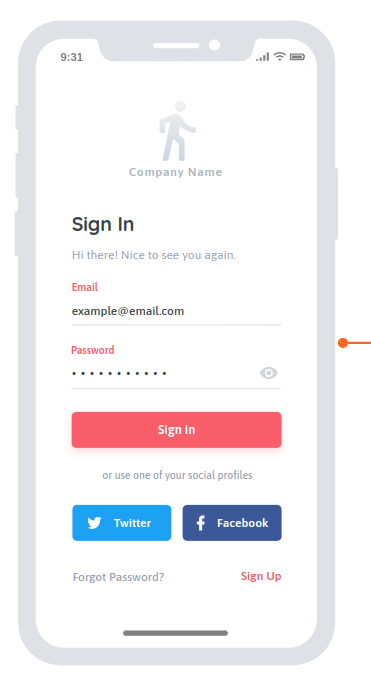
\includegraphics[width=20em]{./graphics/login_Mockup.png}
        \centering
        \caption{Mock up Login}
        \label{fig:loginMockup}
    \end{figure}

    \begin{figure}[H]
        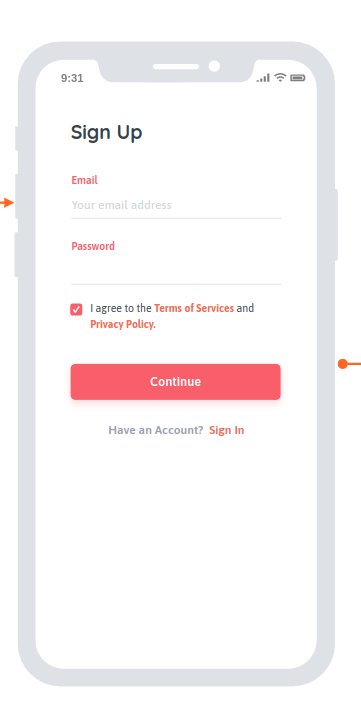
\includegraphics[width=20em]{./graphics/register_Mockup.png}
        \centering
        \caption{Mock up Register}
        \label{fig:registerMockup}
    \end{figure}
    
    \begin{figure}[H]
        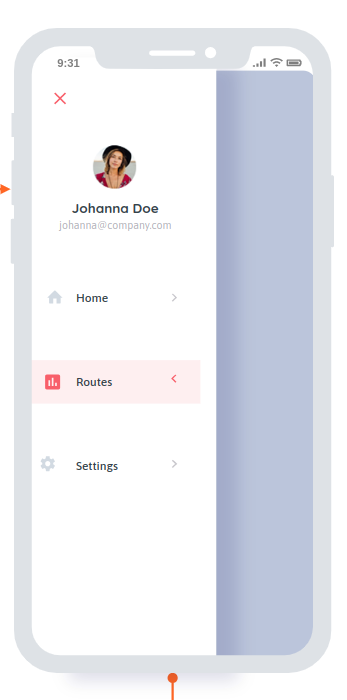
\includegraphics[width=20em]{./graphics/drawer_Mockup.png}
        \centering
        \caption{Mock up Drawer menu}
        \label{fig:DrawerMockup}
    \end{figure}

    \begin{figure}[H]
        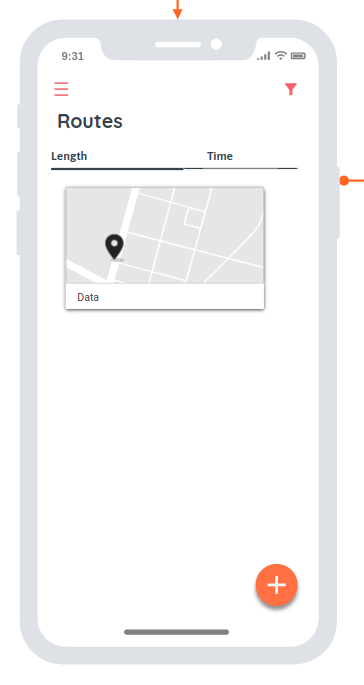
\includegraphics[width=20em]{./graphics/routeView_Mockup.png}
        \centering
        \caption{Mock up Route View}
        \label{fig:routeViewMockup}
    \end{figure}

    \begin{figure}[H]
        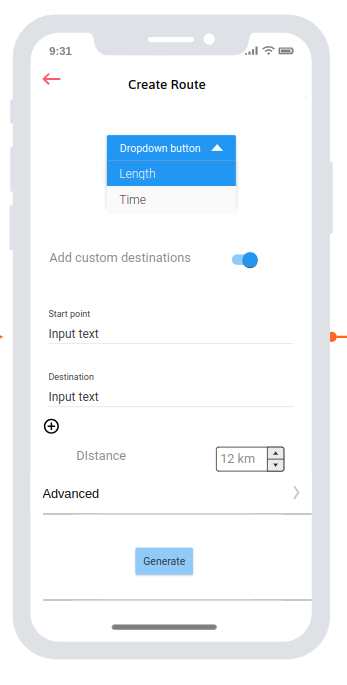
\includegraphics[width=20em]{./graphics/createRoute_Mockup.png}
        \centering
        \caption{Mock up Route Create}
        \label{fig:createRouteMockup}
    \end{figure}

    \begin{figure}[H]
        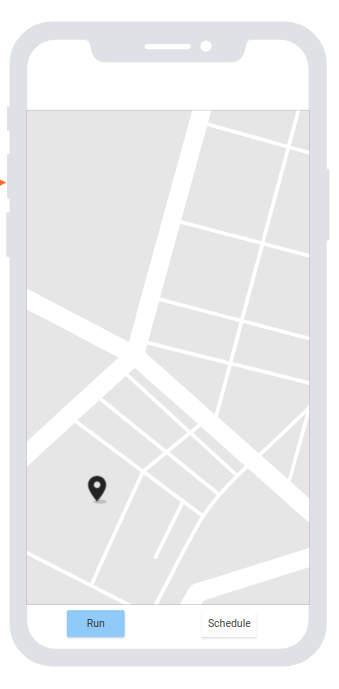
\includegraphics[width=20em]{./graphics/route_Mockup.png}
        \centering
        \caption{Mock up Route}
        \label{fig:routeMockup}
    \end{figure}

    \pagebreak

    \section{Proof of Concept}

    Na het ontwerp volgt de fase van ontwikkeling en implementatie. Hier wordt een Proof of Concept ontwikkeld, 
    bestaande uit zowel een online backend als een mobiele applicatie.

    \vspace{1cm}


    De code is beschikbaar op Github. 

    \vspace{1cm}

    De frontend \url{https://github.com/LaurensDM/RunnerApp}.
    
    \vspace{1cm}

    De backend \url{https://github.com/LaurensDM/RunnerApp-API}

    \subsection{Frontend}

    react-native-paper en react-native-navigation worden gebruikt voor styling en navigatie. 
    De applicatie is opgedeeld in verschillende componenten, 
    zoals HomeScherm, RouteScherm, SettingsScherm, SavedRoutesScherm, RouteCreateScherm en RouteDetailsScherm. 
    De navigatie tussen de verschillende schermen gebeurt via een drawer menu. 
    De applicatie maakt gebruik van Auth0 voor authenticatie en autorisatie. 
    De gebruiker kan inloggen met zijn e-mail en wachtwoord en wordt doorgestuurd naar het HomeScherm. 
    Gegevens worden opgeslagen in de lokale opslag van de mobiele applicatie via AsyncStorage.

    \vspace{1cm}


    Om een route te genereren is een internetverbinding nodig, 
    maar een gebruiker kan een bestaande route terug ophalen en bekijken zonder internetverbinding. Deze exacte route kan dan opnieuw gelopen worden. Aanpassingen aan de route kunnen enkel gebeuren met een internetverbinding.

    \vspace{1cm}

    
    Hier is een overzicht van de verschillende schermen van de applicatie:

    \vspace{1cm}

    
    Eerst wordt de gebruiker gevraagd om in te loggen. Hierbij wordt de gebruiker doorverwezen naar een browser waar Auth0 de authenticatie regelt.

    \begin{figure}[htbp]
        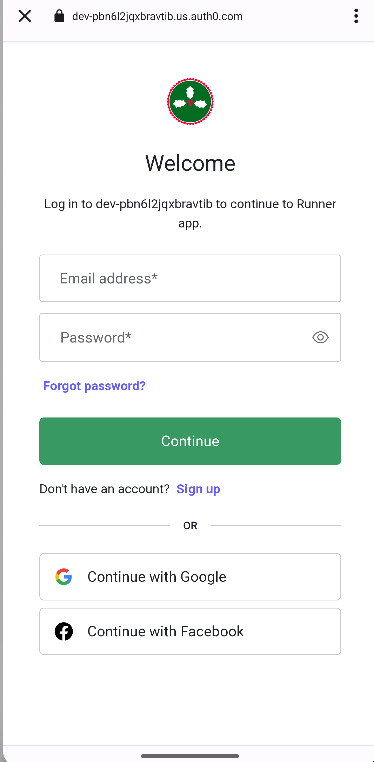
\includegraphics[width=20em]{./graphics/login.png}
        \centering
        \caption{Login}
        \label{fig:login}
    \end{figure}

    Vervolgens komt de gebruiker op het Home Scherm terecht. Voor de Proof of Concept staat hiet niet veel, 
    maar in de toekomst kan hier data van de gebruiker getoond worden.

    \begin{figure}[H]
        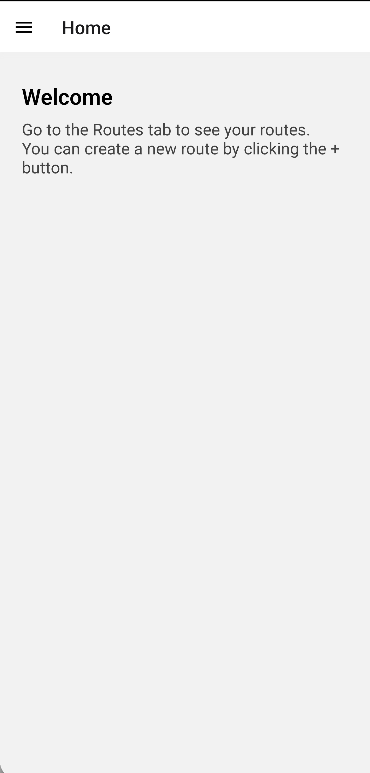
\includegraphics[width=20em]{./graphics/home.png}
        \centering
        \caption{Home}
        \label{fig:home}
    \end{figure}

    Via het drawer menu kan de gebruiker navigeren naar de verschillende schermen van de applicatie.

    \begin{figure}[H]
        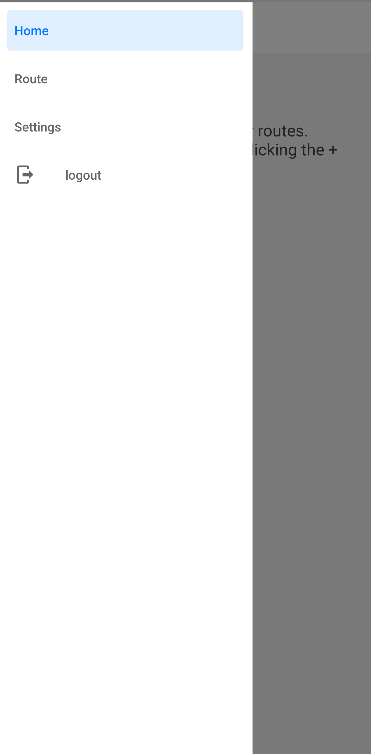
\includegraphics[width=20em]{./graphics/drawer.png}
        \centering
        \caption{Drawer}
        \label{fig:drawer}
    \end{figure}

    Op het Route Overzicht scherm kan de gebruiker de opgeslagen routes bekijken en beheren. Het is mogelijk op een route te selecteren om de details te bekijken. Hierbij wordt de route opgehaald uit de lokale opslag van de mobiele applicatie. Het is hier mogelijk om een nieuwe route te genereren met dezelfde parameters als de geselecteerde route, of om de route gewoon opnieuw te lopen.

    \vspace{1cm}


    Er is een onderscheid tussen routes gebaseerd op afstand en tijd. Er is geen verschil in de route die wordt gegenereerd. Bij een route op tijd wordt de afstand berekent op basis van de loopsnelheid van de gebruiker. Deze kan ingesteld worden in de Settings van de applicatie.

    \begin{figure}[H]
        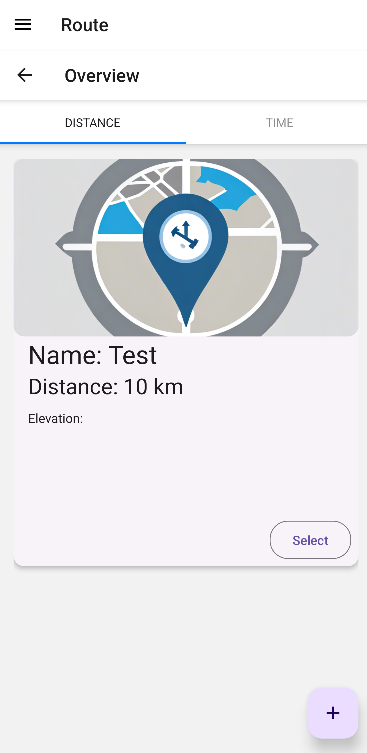
\includegraphics[width=20em]{./graphics/routes.png}
        \centering
        \caption{Routes}
        \label{fig:routes}
    \end{figure}

    Er is een plus knop die de gebruiker naar het Route Creatie scherm brengt. Hier kan de gebruiker een route genereren op basis van specifieke parameters. Eens alle parameters zijn ingevuld, kan de gebruiker de route genereren en wordt deze doorgestuurd naar het Route scherm.

    \begin{figure}[H]
        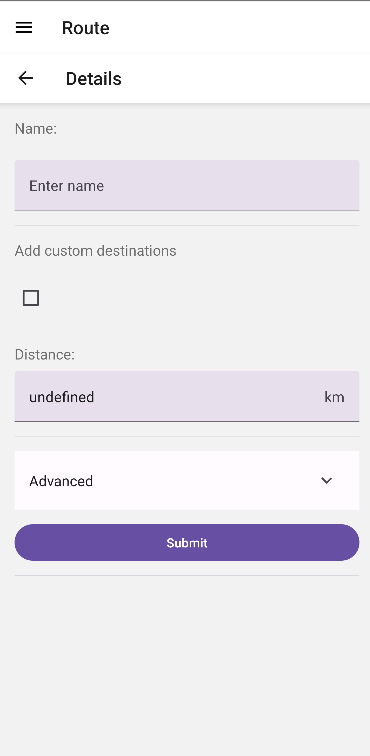
\includegraphics[width=20em]{./graphics/create.png}
        \centering
        \caption{Create Route}
        \label{fig:createRoute}
    \end{figure}

    Op het Route scherm kan de gebruiker de details van de gegenereerde route bekijken. Hier kan de gebruiker ook een weerbericht opvragen voor de route. De gebruiker kan de route opslaan om later te lopen of meteen starten.

    \begin{figure}[H]
        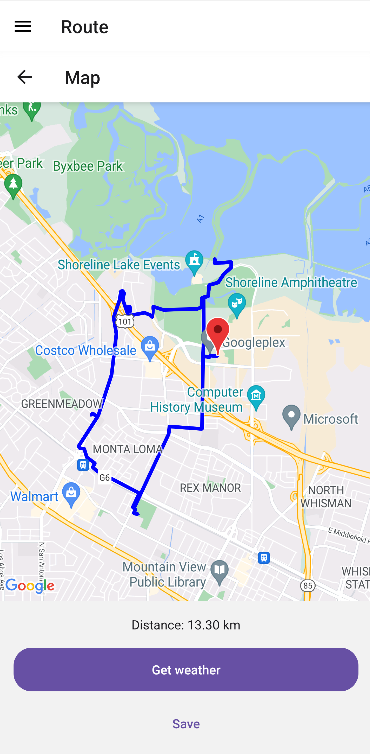
\includegraphics[width=20em]{./graphics/route.png}
        \centering
        \caption{Route}
        \label{fig:route}
    \end{figure}

    \begin{figure}[H]
        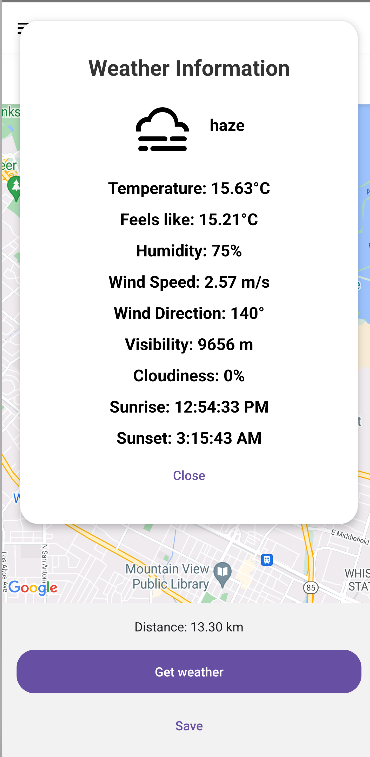
\includegraphics[width=20em]{./graphics/weather.png}
        \centering
        \caption{Weer}
        \label{fig:weather}
    \end{figure}

    Er is ook een instellingen scherm waar de gebruiker de instellingen van de applicatie kan aanpassen, zoals de loopsnelheid.

    \begin{figure}[H]
        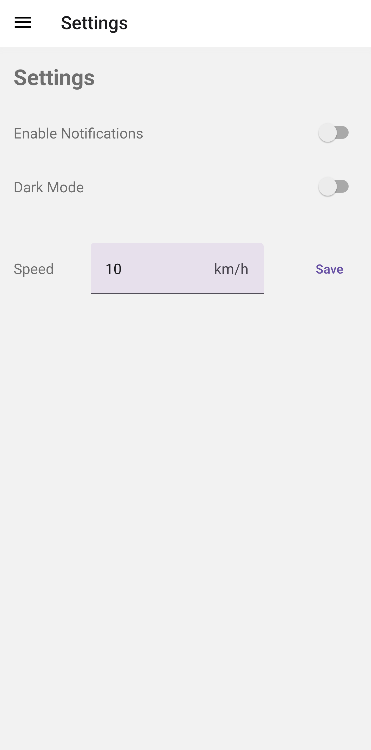
\includegraphics[width=20em]{./graphics/settings.png}
        \centering
        \caption{Instellingen}
        \label{fig:settings}
    \end{figure}


    \subsection{Backend}
    
    De backend is ontwikkeld met behulp van Node.js en Express.js en communiceert met de frontend via een RESTful API. 
    Auth0 wordt gebruikt voor authenticatie en autorisatie.
    De backend communiceert verder met de Overpass API, Google Maps API en OpenWeatherMap API voor het genereren van looproutes en het opvragen van weersverwachtingen.

    \vspace{1cm}

    
    Hier is een overzicht van de verschillende endpoints van de API. Er zijn andere endpoints ingesteld, maar de enigen die momenteel werken zijn de endpoints voor het genereren van een route en het ophalen van een weersvoorspelling.
    \begin{itemize}
        \item POST /api/route/
        \item POST /api/weather/
    \end{itemize}
  
    \vspace{1cm}


    Deze zijn de andere endpoints die ingesteld zijn, maar niet werken.
    \begin{itemize}
        \item POST /api/
        \item GET /api/user/
        \item GET /api/route/
        \item PUT /api/route/:id
        \item DELETE /api/route/:id
    \end{itemize}

    \vspace{1cm}

    
    Het genereren van een route gebeurt in verschillende stappen. 
    De API krijgt eerst de nodige data binnen van de frontend, zoals de locatie van de gebruiker, de gewenste afstand of tijd van de route en verdere geavanceerde opties. 
    De API valideert eerst of alle nodige parameters aanwezig zijn met behulp van express-validator. 

    \vspace{1cm}

    Vervolgens wordt een functie aangeroepen die de Overpass API aanspreekt om tussenpunten te genereren op basis van de gegeven parameters. 
    Functies die de Overpass API en Google Maps API aanspreken zijn gedefinieerd in een helpers folder, zodat er makkelijk integraties met andere platformen kunnen worden toegevoegd. 

    \vspace{1cm}

    Met de tussenpunten wordt een for-loop gestart die de afstand tussen de tussenpunten berekent. Ook wordt hier de hoogte van de verschillende tussenpunten berekent en worden tussenpunten gefilterd 
    op basis van de gewenste hoogte die de gebruiker heeft gespecifieerd. Dit gebeurt aan de hand van de Google Maps API.
    Als de afstand tussen de tussenpunten groter is dan de gewenste afstand van de route,
    wordt de loop beëindigd zonder dat alle tussenpunten zijn inbegrepen. 

    \vspace{1cm}

    In het geval dat er geen tussenpunten zijn teruggevonden, wordt een tussenpunt gegenereerd op basis van de locatie van de gebruiker, die zich dan op een aantal kilometers van de startlocatie bevindt. 
    De route wordt teruggegeven aan de frontend.

    \pagebreak

Dit is de code die verantwoordelijk is voor het genereren van de route.

\begin{lstlisting}
    async function generateRunningRoute({ startPoint, endPoint, waypoints, distance, advancedOptions }: RouteProps) {

    const generatedWaypoints = await getGeneratedWaypoints(distance!, startPoint, advancedOptions.poiTypes, advancedOptions.surfaceType);


    const runningRouteWaypoints: Waypoint[] = [];

    generatedWaypoints.sort((a, b) => {
        return calculateDistance(startPoint, a) - calculateDistance(startPoint, b);
    });

    let accumulatedDistance = 0;


    const elevationWaypoints = await calculateElevation([startPoint, ...generatedWaypoints.slice(0, 510), endPoint]);

    const filteredWaypoints = elevationWaypoints.filter((waypoint) => {
        const elevationChange = Math.abs(waypoint.elevation - elevationWaypoints[0].elevation); // Assuming startPoint elevation as reference
        if (elevationChange < 50) { // Adjust thresholds for flat, medium, and steep as needed
            return advancedOptions.height === 'flat';
        } else if (elevationChange < 100) {
            return advancedOptions.height === 'medium';
        } else {
            return advancedOptions.height === 'steep';
        }
    });

    const accumulatedWaypoints = filteredWaypoints != undefined && filteredWaypoints.length > 2 ? filteredWaypoints : generatedWaypoints;
    const allWaypoints = [...waypoints.sort((a, b) => calculateDistance(startPoint, a) - calculateDistance(startPoint, b)), ...accumulatedWaypoints];
    
    console.log('All waypoints:', allWaypoints.length);
    console.log(allWaypoints);
    
    const waypointLimit = 25;
    let timeOut = 0;
    if (allWaypoints.length === 0) {
        let currentPoint = startPoint;
        while (accumulatedDistance < distance * 1000) { // Convert km to meters
            // Find the next point along the route
            const nextPoint = findNextPoint(currentPoint, endPoint, distance * 1000 - accumulatedDistance, (distance / 6 * 1000));
            const calculatedDistance = calculateDistance(currentPoint, nextPoint);

            // Add the next point to the running route waypoints
            runningRouteWaypoints.push(nextPoint);
            accumulatedDistance += calculatedDistance;

            // Update currentPoint for the next iteration
            console.log(currentPoint);

            currentPoint = nextPoint;
            if (timeOut > 1000 || runningRouteWaypoints.length === 4) {
                break;
            }
            timeOut++;
        }
    } else {
        for (let i = 0; i < allWaypoints.length; i++) {
            const previousWaypoint = i === 0 ? startPoint : allWaypoints[i - 1];
            const waypoint1 = allWaypoints[i];
            const calculatedDistance = calculateDistance(previousWaypoint, waypoint1);
            const distanceToEnd = calculateDistance(waypoint1, endPoint);
            // accumulatedDistance += (accumulatedDistance + calculatedDistance) > distance *1000 ? 0 : calculatedDistance;
            if ((accumulatedDistance + calculatedDistance) > distance * 1000 || accumulatedDistance + distanceToEnd > distance * 1000) {
                accumulatedDistance += 0;
            } else {
                accumulatedDistance += calculatedDistance;
            }

            if (accumulatedDistance <= distance * 1000) { // Convert km to meters
                runningRouteWaypoints.push(waypoint1);
            } else {
                console.log(accumulatedDistance);
                break;
            }

            //Only 25 waypoints are allowed in a single request
            if (runningRouteWaypoints.length === waypointLimit) {
                console.log(accumulatedDistance);
                break;
            }
        }
    }
    runningRouteWaypoints.sort((a, b) => {
        return calculateDistance(a, endPoint) - calculateDistance(b, endPoint);
    });

    console.log('Running route waypoints:', runningRouteWaypoints.length);

    console.log(runningRouteWaypoints);



    // Generate route using Google Maps Directions API
    try {
        const createdRoute = await generateGoogleRoute(startPoint, endPoint, runningRouteWaypoints);
        return createdRoute.routes;
    } catch (error: any) {
        console.error('Error fetching route:', error.response.data);
        return null;
    }
}
\end{lstlisting}

Deze functie genereert een hardlooproute op basis van een aantal parameters. Waaronder een startpunt, een eindpunt, tussenpunten, de afstand van de route en geavanceerde opties.

\vspace{1cm}

De functie begint met het ophalen van gegenereerde tussenpunten met behulp van de getGeneratedWaypoints functie. Deze functie roept de Overpass API aan en genereert tussenpunten op basis van de gegeven parameters.
Er worden maximum 50 tussenpunten gegenereerd per parameter.
Deze gegenereerde tussenpunten worden vervolgens gesorteerd op basis van hun afstand tot het startpunt. De afstand wordt berekend met behulp van de calculateDistance functie.

\vspace{1cm}

Vervolgens wordt de hoogte van de route berekend met behulp van de calculateElevation functie. Deze functie roept de Google Maps Elevation API aan en berekent de hoogte van de verschillende tussenpunten. 
Hieraan worden enkel 510 tussenpunten meegegeven, omdat de Google Maps Elevation API een limiet heeft van 512 punten per aanvraag.
Er wordt gekeken naar het hoogteverschil tussen de verschillende tussenpunten en op basis daarvan worden de tussenpunten gefilterd. Dit wordt gedaan op basis van de geavanceerde opties die zijn meegegeven.

\vspace{1cm}

De gefilterde tussenpunten worden toegevoegd aan de lijst met alle tussenpunten. Als er geen tussenpunten zijn gegenereerd, worden er nieuwe tussenpunten gecreëerd door middel van de findNextPoint functie. 
Deze functie zoekt naar het volgende punt langs de route en voegt dit toe aan de lijst met tussenpunten. In totaal worden 4 tussenpunten gegenereerd die verspreid zijn in een radius die gelijk is aan de afstand van de route.
Dit wordt herhaald totdat de totale afstand van de route overeenkomt met de gewenste afstand of tot er 4 tussenpunten berekent zijn.

\vspace{1cm}

Als er wel tussenpunten zijn, dan worden deze toegevoegd aan de lijst met tussenpunten. Er wordt gekeken naar de afstand tussen de tussenpunten en of deze afstand past binnen de gewenste afstand van de route. 
Als de afstand tussen twee tussenpunten te groot is, wordt deze tussenpunt niet toegevoegd aan de lijst.

\vspace{1cm}

Er mag maximaal gebruik worden gemaakt van 25 tussenpunten in een enkele aanvraag. Als er meer tussenpunten zijn dan dit, dan worden alleen de eerste 25 tussenpunten gebruikt.
Dit is de limiet van de Google Maps Directions API.

\vspace{1cm}

Als de lijst met tussenpunten compleet is, dan wordt er met behulp van de Google Maps Directions API een route gegenereerd. 
Deze route wordt teruggegeven als resultaat van de functie. Als er een fout optreedt bij het ophalen van de route, dan wordt er null teruggegeven.
\chapter{\IfLanguageName{dutch}{Resultaten}{Results}}%
\label{ch:resultaten}

In dit hoofdstuk worden de resultaten van de route generatie besproken. 
Volgende routes worden gegenereerd:
\begin{itemize}
    \item 5 km route
    \item 10 km route
    \item 50 km route
    \item 100 km route
\end{itemize}
\section{Zonder geavanceerde opties}

\subsection{5 km route}

\begin{figure}[H]
    \centering
    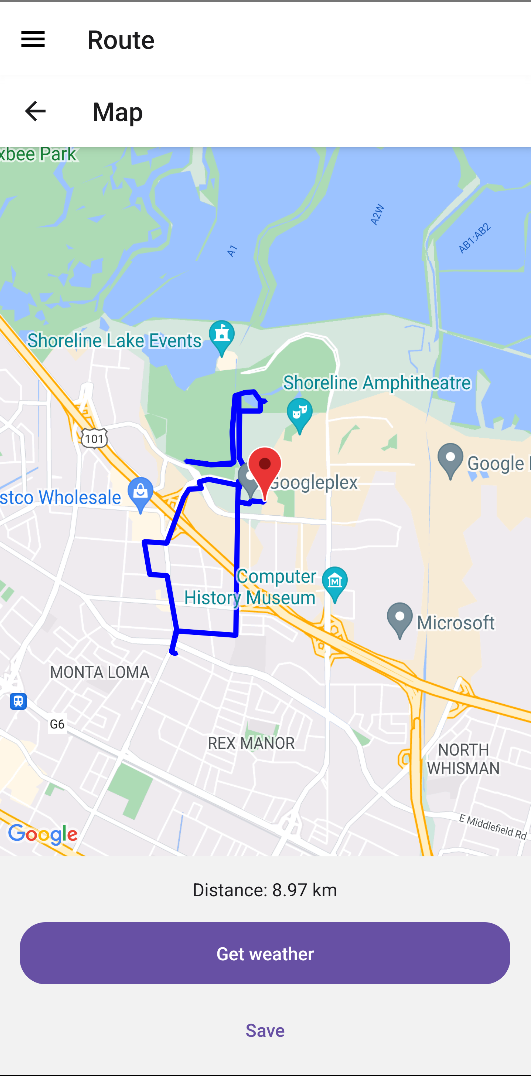
\includegraphics[width=20em]{5km_route}
    \caption{5 km route}
    \label{fig:5km_route}

\end{figure}

De gegenereerde route is 8.97 km lang, dit is langer dan de gevraagde 5 km. Dit komt omdat de route steeds elk punt van de route probeert te verbinden met de kortste afstand. Dit kan lijden tot een langere route dan gevraagd.
De vorm van de route is vooral een lus, maar er zijn ook enkele stukken die heen en terug gaan.

Uitgedruk in procent is de route 79.4\% langer dan gevraagd.
\subsection{10 km route}

\begin{figure}[H]
    \centering
    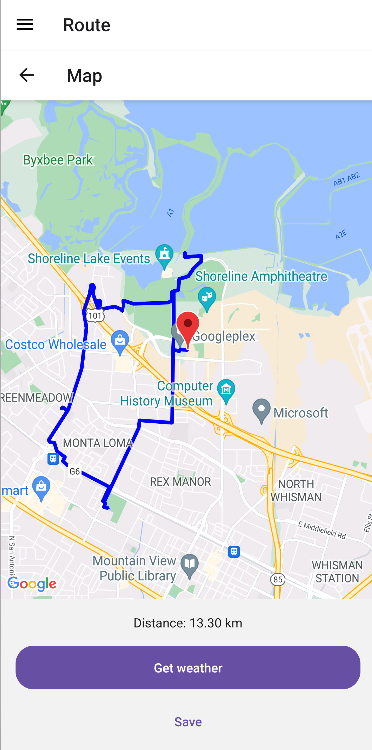
\includegraphics[width=20em]{10km_route}
    \caption{10 km route}
    \label{fig:10km_route}

\end{figure}

De gegenereerde route is 13.30 km lang, dit is langer dan de gevraagde 10 km. De vorm van de route lijkt al meer op een volledige lustructuur, maar er zijn nog steeds enkele stukken die heen en terug gaan.

Uitgedruk in procent is de route 33\% langer dan gevraagd.

\subsection{50 km route}

\begin{figure}[H]
    \centering
    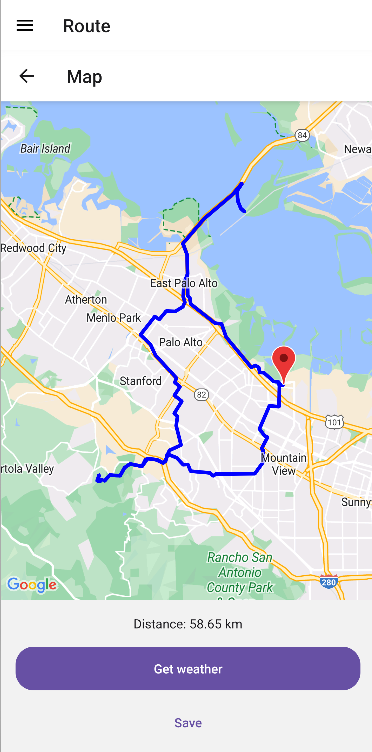
\includegraphics[width=20em]{50km_route}
    \caption{50 km route}
    \label{fig:50km_route}

\end{figure}

De gegenereerde route is 58.65 km lang, dit is ook langer dan gevraagd. De vorm van de route is een volledige lus, met 2 'takken' die hieruit springen, die heen en terug gaan.

Uitgedruk in procent is de route 17.3\% langer dan gevraagd.

\subsection{100 km route}

\begin{figure}[H]
    \centering
    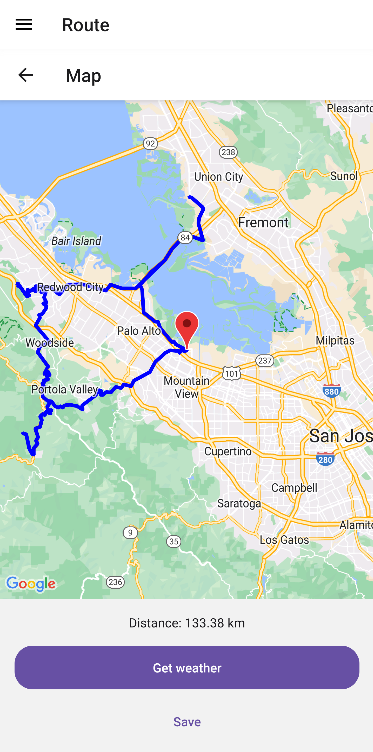
\includegraphics[width=20em]{100km_route}
    \caption{100 km route}
    \label{fig:100km_route}

\end{figure}

De gegenereerde route is 133.38km lang, dit is langer dan gevraagd. Ook hier is de vorm van de route een volledige lus, met nu 3 'takken' die hieruit springen, die heen en terug gaan.

Uitgedruk in procent is de route 33.4\% langer dan gevraagd.

\pagebreak

\subsection{Algemeen}

De routes die gegenereerd worden zonder geavanceerde opties zijn de meest eenvoudige routes. De routes zijn vooral lussen, met enkele stukken die heen en terug gaan. De routes zijn vaak langer dan gevraagd.

Gemiddeld is de route 40.8\% langer dan gevraagd.

\section{Met geavanceerde opties}

Als geavanceerde opties worden de volgende opties ingesteld:
\begin{itemize}
    \item Elevation: Medium
    \item Underground: ground
    \item Points of interest: park, running, path, footway, tree, viewpoint
\end{itemize}

\subsection{5 km route}

\begin{figure}[H]
    \centering
    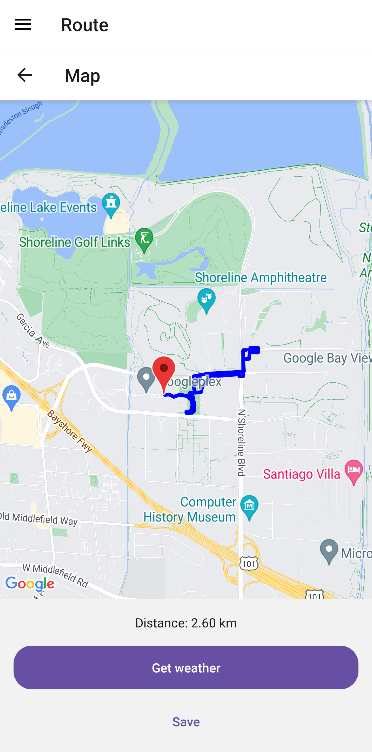
\includegraphics[width=20em]{5km_route_geavanceerd}
    \caption{5 km route met geavanceerde opties}
    \label{fig:5km_route_geavanceerd}

\end{figure}

De gegenereerde route is 2.60 km lang, dit is bijna de helft van de gevraagde 5km. De vorm van de route bestaat enkel uit stukken die heen en terug gaan.

Uitgedruk in procent is de route 48\% korter dan gevraagd.

\subsection{10 km route}

\begin{figure}[H]
    \centering
    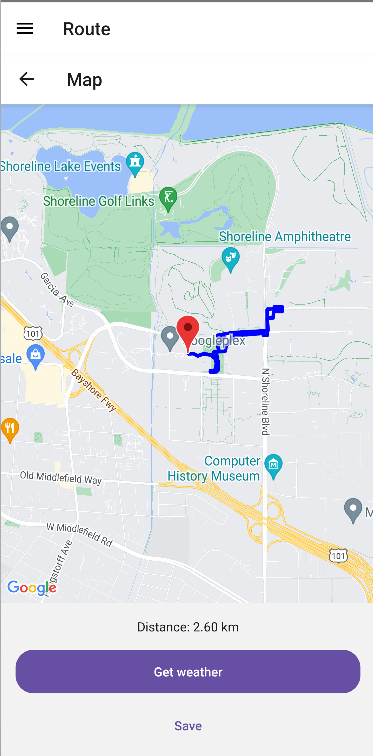
\includegraphics[width=20em]{10km_route_geavanceerd}
    \caption{10 km route met geavanceerde opties}
    \label{fig:10km_route_geavanceerd}

\end{figure}

De gegenereerde route is 2.60 km lang, dit is veel korter dan de gevraagde 10km. De route lijkt dezelfde te zijn als bij 5km.

Uitgedruk in procent is de route 74\% korter dan gevraagd.

\subsection{50 km route}

\begin{figure}[H]
    \centering
    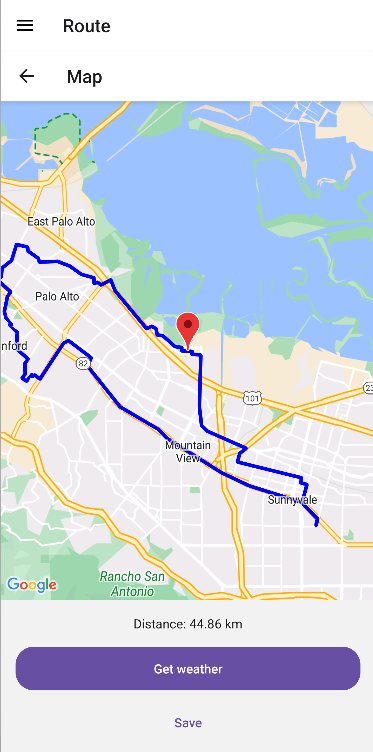
\includegraphics[width=20em]{50km_route_geavanceerd}
    \caption{50 km route met geavanceerde opties}
    \label{fig:50km_route_geavanceerd}

\end{figure}

De gegenereerde route is 44.86 km lang, dit is een beetje korter dan de gevraagde 50km. Deze route is een volledige lus.

Uitgedruk in procent is de route 10.28\% korter dan gevraagd.

\subsection{100 km route}

\begin{figure}[H]
    \centering
    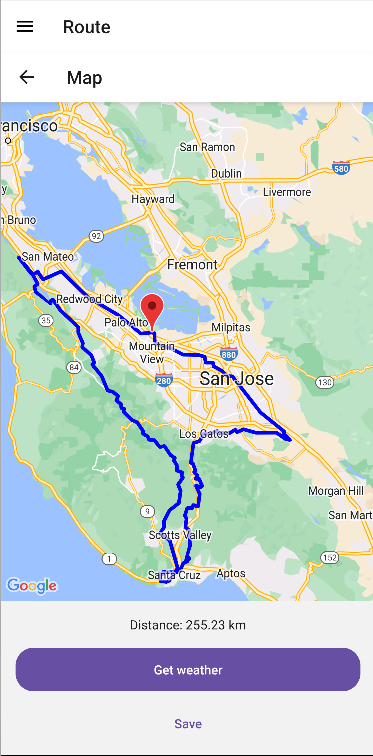
\includegraphics[width=20em]{100km_route_geavanceerd}
    \caption{100 km route met geavanceerde opties}
    \label{fig:100km_route_geavanceerd}
\end{figure}

De gegenereerde route is 255.23 km lang, dit is enorm veel langer dan de gevraagde 100 km. Deze route lijkt echter wel een volledige lus te zijn.

Uitgedruk in procent is de route 155.23\% langer dan gevraagd.


\pagebreak

\subsection{Algemeen}

De routes die gegenereerd worden met geavanceerde opties zijn doorgaans korter dan de gevraagde afstand. Met uitzondering de route van 100 km, deze is veel langer dan gevraagd.
De routes bestaan meer uit lussen. De variatie in afstand tussen de routes ligt aan de punten die de OverPass API teruggeeft en is sterk afhankelijk van de locatie van de gebruiker.

Gemiddeld is de route 41.4\% korter dan gevraagd.

\section{Met zelf gekozen punten}

Als zelf gekozen punten worden de volgende punten ingesteld:
\begin{itemize}
    \item Start: HOGENT campus Schoonmeersen, Valentin Vaerwyckweg, Ghent, Belgium
    \item Einde: Overpoortstraat, Ghent, Belgium
    \item Punt: Gravensteen, Sint-Veerleplein, Ghent, Belgium
\end{itemize}

De geavanceerde opties worden behouden van vorige sectie.

\subsection{5 km route}

\begin{figure}[H]
    \centering
    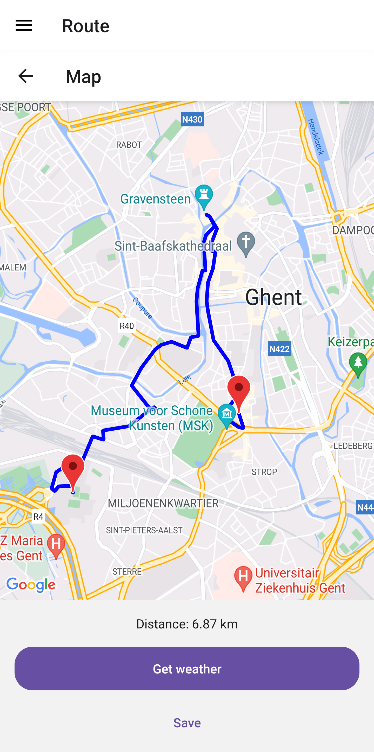
\includegraphics[width=20em]{5km_route_zelf}
    \caption{5 km route met zelf gekozen punten}
    \label{fig:5km_route_zelf}

\end{figure}

De gegenereerde route is 6.87 km lang, dit is een beetje langer dan de gevraagde 5 km.

Uitgedruk in procent is de route 37.4\% langer dan gevraagd

\subsection{10 km route}

\begin{figure}[H]
    \centering
    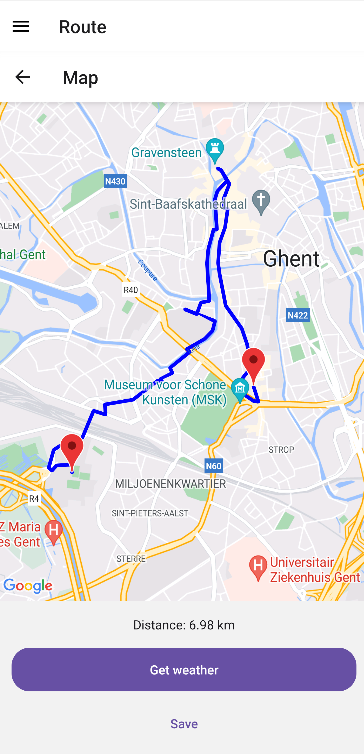
\includegraphics[width=20em]{10km_route_zelf}
    \caption{10 km route met zelf gekozen punten}
    \label{fig:10km_route_zelf}

\end{figure}

De gegenereerde route is 6.98 km lang, dit is korter dan de gevraagde 10 km en is bijna hetzelfde als de 5 km route.

Uitgedruk in procent is de route 30.2\% korter dan gevraagd.

\subsection{50 km route}

\begin{figure}[H]
    \centering
    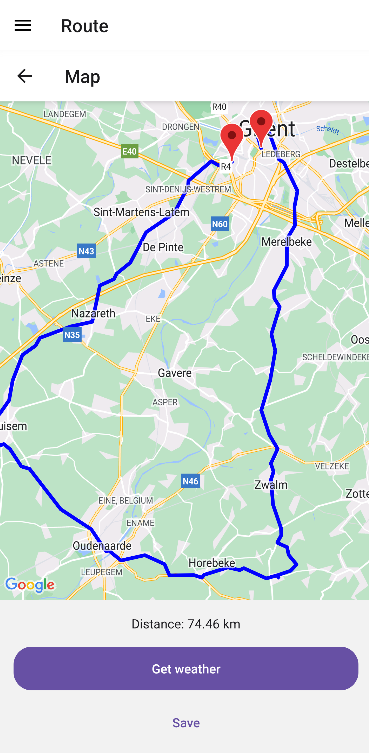
\includegraphics[width=20em]{50km_route_zelf}
    \caption{50 km route met zelf gekozen punten}
    \label{fig:50km_route_zelf}

\end{figure}

De gegenereerde route is 74.46 km lang, dit is langer dan de gevraagde 50 km.

Uitgedruk in procent is de route 48.9\% langer dan gevraagd.

\subsection{100 km route}

\begin{figure}[H]
    \centering
    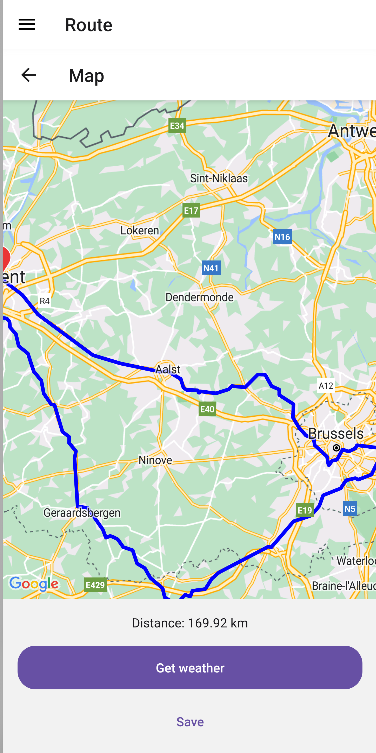
\includegraphics[width=20em]{100km_route_zelf}
    \caption{100 km route met zelf gekozen punten}
    \label{fig:100km_route_zelf}

\end{figure}

De gegenereerde route is 169.92 km lang, dit is langer dan de gevraagde 100 km.

Uitgedruk in procent is de route 69.92\% langer dan gevraagd


\pagebreak

\subsection{Algemeen}

De routes die gegenereerd worden met zelf gekozen punten zijn doorgaans langer dan de gevraagde afstand. De variatie in afstand tussen de routes ligt aan de punten die de OverPass API teruggeeft en is sterk afhankelijk van de locatie van de gebruiker.

Gemiddeld is de route 46.6\% langer dan gevraagd.

\section{Besluit}

De routes die gegenereerd worden zonder geavanceerde opties zijn de meest eenvoudige routes. De routes zijn vooral lussen, met enkele stukken die heen en terug gaan. De routes zijn ook langer dan gevraagd.
Doorgaans zullen routes die berekent worden op deze manier het minst variabel zijn.

De routes die gegenereerd worden met geavanceerde opties zijn doorgaans korter dan de gevraagde afstand. Met uitzondering de route van 100 km, deze is veel langer dan gevraagd.
De routes bestaan meer uit lussen. De variatie in afstand tussen de routes ligt aan de punten die de OverPass API teruggeeft en is sterk afhankelijk van de locatie van de gebruiker.
Er werd een poging gedaan om de lengte van de route te beperken in het algoritme, maar deze is niet altijd succesvol. Dit komt omdat de afstand tussen punten in het algoritme in vogelvlucht wordt berekend en niet over de weg.
De kwaliteit van deze routes is sterk afhankelijk van de geavanceerde opties die de gebruiker kiest en de locatie van de gebruiker.

De routes die gegenereerd worden met zelf gekozen punten zijn doorgaans langer dan de gevraagde afstand. 
De variatie in afstand tussen de routes ligt hier ook aan de punten die de OverPass API teruggeeft en is sterk afhankelijk van de locatie van de gebruiker. 
Het is echter minder extreem en de genereerde routes lijken van betere kwaliteit te zijn dan de routes die gegenereerd worden met geavanceerde opties, zonder zelf gedefinieerde punten.

Het is steeds mogelijk om op de terug te knop te drukken en een nieuwe route te genereren, de parameters die ingesteld zijn blijven behouden. Dit kan handig zijn als de gebruiker niet tevreden is met de gegenereerde route.








\chapter{\IfLanguageName{dutch}{Kostenanalyse}{Cost analyses}}%
\label{ch:kostenanalyse}

In dit hoofdstuk wordt een kostenanalyse uitgevoerd voor de ontwikkeling en het onderhoud van de Proof of Concept.

\section{Kosten voor het publiceren van de Proof of Concept}%

De kosten voor de publicatie van de Proof of Concept zijn afhankelijk van het platform waarop de applicatie wordt gepubliceerd. In dit geval wordt de applicatie gepubliceerd op zowel de Google Play Store als de Apple App Store. Beide platformen hanteren eenmalige kosten voor het publiceren van een applicatie.

De backend moet ook worden gehost op een server. De kosten voor het hosten van de backend zijn afhankelijk van de gekozen hostingprovider en het gekozen hostingplan. 

Aangezien deze kosten zeer variabel zijn en afhangen van de manier waarop de applicatie wordt gepubliceerd en gehost, is het moeilijk om een exact bedrag vast te stellen. Dus zal dit onderdeel van de kostenanalyse worden uitgesloten.

\section{Kosten voor de tools van de Proof of Concept}%

De Proof of Concept maakt gebruik van verschillende tools en services om de functionaliteit van de applicatie te ondersteunen. Deze tools en services hebben elk hun eigen kostenstructuur.

\subsection{Google Maps API}%

De Google Maps API is een belangrijk onderdeel van de Proof of Concept, omdat het de mogelijkheid biedt om kaarten en locatiegegevens te integreren in de applicatie. De Google Maps API hanteert een pay-as-you-go model, waarbij de kosten afhankelijk zijn van het gebruik van de API.

De kosten voor het gebruik van de Google Maps API zijn als volgt:

\begin{itemize}
    \item \$5 per 1000 routeberekeningen
    \item \$0,50 per 1000 geocodingverzoeken
\end{itemize}

Er wordt gratis \$200 aan credits gegeven per maand. 
Dus kunnen er 40.000 routeberekeningen per maand worden gedaan.

De kosten voor het gebruik van de Google Maps API kunnen variëren afhankelijk van het aantal gebruikers en het gebruik van de applicatie. Voor de Proof of Concept zijn de kosten voor het gebruik van de Google Maps API echter verwaarloosbaar, omdat het aantal gebruikers en het gebruik van de applicatie beperkt is.

\subsection{Overpass API}%

De Overpass API is een open-source API die wordt gebruikt om gegevens over OpenStreetMap te extraheren. De Overpass API is gratis te gebruiken en er zijn geen kosten verbonden aan het gebruik ervan.

Echter is het belangrijk om te vermelden dat de Overpass API een limiet heeft op het aantal verzoeken dat per dag kan worden gedaan. Als deze limiet wordt overschreden, kan de toegang tot de API worden geblokkeerd. Deze limiet is ongeveer 10.000 verzoeken per dag en downloads minder dan 1 GB per dag. Voor de Proof of Concept zijn deze limieten echter niet relevant, omdat het aantal verzoeken dat wordt gedaan binnen deze limieten valt. Om meer verzoeken te kunnen doen, kan er een eigen Overpass API server worden opgezet. Deze kosten zijn echter niet meegenomen in deze kostenanalyse.

\subsection{OpenWeatherMap API}%

De OpenWeatherMap API is een open-source API die wordt gebruikt om weergegevens te integreren in de applicatie. De OpenWeatherMap API hanteert een freemium model, waarbij een gratis abonnement beschikbaar is met beperkte functionaliteit en een betaald abonnement met meer geavanceerde functies. 

Het gratis abonnement van de OpenWeatherMap API biedt de volgende functies:

\begin{itemize}
    \item 60 verzoeken per minuut
    \item 1 miljoen verzoeken per maand
    \item 5-daagse weersvoorspelling
    \item Huidige weersomstandigheden
\end{itemize}

Voor de Proof of Concept zijn de kosten voor het gebruik van de OpenWeatherMap API echter verwaarloosbaar, omdat het aantal verzoeken dat wordt gedaan binnen de limieten van het gratis abonnement valt. Ook de extra functies van het betaalde abonnement zijn niet nodig. Voor meer gebruikers kan het echter nodig zijn om over te schakelen naar een betaald abonnement.  Het is 0.0014 euro per API call over de limiet.

\subsection*{Auth0}

Auth0 is een tool die wordt gebruikt voor authenticatie en autorisatie in de Proof of Concept. Auth0 hanteert een freemium model, waarbij een gratis abonnement beschikbaar is met beperkte functionaliteit en een betaald abonnement met meer geavanceerde functies.

Met dit gratis abonnement kunnen er 7500 actieve gebruikers per maand worden geregistreerd. Voor de Proof of Concept zijn de kosten voor het gebruik van Auth0 echter verwaarloosbaar, omdat het aantal gebruikers en het gebruik van de applicatie beperkt is. Voor meer gebruikers kan het echter nodig zijn om over te schakelen naar een betaald abonnement.

\subsection*{Hosting}

Voor de hosting kan gebruik worden gemaakt van Render. Render biedt een gratis plan aan voor kleine applicaties. Met dit plan zou het mogelijk zijn om de backend van de Proof of Concept te hosten. Er kan maar een maximum van 40.000 routeberekeningen per maand worden gedaan voor Google Maps. Deze Render server is voldoende voor dit aantal api calls. Het is niet aanbevolen om dit gratis plan te gebruiken voor een productieomgeving. Voor meer gebruikers kan het nodig zijn om over te schakelen naar een betaald abonnement.

\section{Conclusie}%

De kosten voor de publicatie van de Proof of Concept zijn afhankelijk van het platform waarop de applicatie wordt gepubliceerd en de hostingprovider die wordt gebruikt voor de backend. De kosten voor de tools en services die worden gebruikt in de Proof of Concept zijn verwaarloosbaar, omdat het aantal gebruikers en het gebruik van de applicatie beperkt is. Voor meer gebruikers kunnen de kosten echter toenemen en kan het nodig zijn om over te schakelen naar betaalde abonnementen voor de tools en services die worden gebruikt.

De applicatie is gratis tot 40.000 routeberekeningen per maand. Verder kunnen er maximaal 1 miljoen verzoeken per maand worden gedaan voor een weerbericht op te halen. Als deze limieten worden overschreden, kunnen er extra kosten in rekening worden gebracht. Er is een maximum van 7500 actieve gebruikers.



\chapter{\IfLanguageName{dutch}{Verbeteringen}{Improvements}}%
\label{ch:verbeteringen}

\section{Inleiding}
Dit hoofdstuk biedt een diepgaande verkenning van potentiële verbeteringen voor de applicatie, gebaseerd op een grondige analyse van de literatuur en inzichten verworven tijdens de ontwikkelingsfase. Concreet zijn er 3 concepten die kunnen worden toegevoegd aan de applicatie. Deze concepten zijn: gebruikerservaring, gegevensverzameling en -presentatie, en algemene optimalisaties. Elk concept wordt in detail besproken, met suggesties voor implementatie en mogelijke voordelen voor de gebruiker.

\section{Betere Gebruikers ervaring}

\subsection{Gebruiksvriendelijkheid}

DDe huidige Proof of Concept benut de mogelijkheden voor gebruiksvriendelijkheid nog niet volledig. Er is enkel een focus naar Android systemen, maar het zou mogelijk moeten zijn om de applicatie te laten werken op iOS systemen. Ook is er geen rekening gehouden met de grootte van de schermen van de toestellen. Dit kan worden verbeterd door de applicatie te optimaliseren voor verschillende schermgroottes en besturingssystemen. Dit kan worden gedaan door gebruik te maken van responsive design. Dit is een techniek waarbij de applicatie zich aanpast aan de grootte van het scherm. 

Verder is de applicatie ontwikkeld in het Engels. Dit kan worden uitgebreid naar meerdere talen. Dit kan worden gedaan door gebruik te maken van een vertaalbibliotheek zoals i18n. Dit is een internationale standaard voor het vertalen van applicaties. Ook de uitdrukking van afstanden en snelheden kan worden aangepast aan de lokale standaarden.

\subsection{Ontwerpen}

Ondanks dat er in de literatuur designoverwegingen zijn besproken, zijn deze nog niet geïntegreerd in de Proof of Concept. De applicatie kan worden verbeterd door deze design overwegingen toe te passen. Het implementeren van motivatie- en beloningssystemen, muziekintegratie, gamification en sociale interactie kan de gebruikerservaring verder verrijken. Een beloningssysteem op basis van punten, integratie met populaire muziekstreamingdiensten zoals Spotify, en het toevoegen van gamification-elementen zoals uitdagingen en prestatiebadges kunnen gebruikers stimuleren om actief te blijven en de app regelmatig te gebruiken.

Elk van deze design overwegingen kan worden toegevoegd aan de applicatie. Zo kan er een beloningssysteem worden toegevoegd waarbij de gebruiker punten kan verdienen door te lopen. Deze punten kunnen dan worden gebruikt om een online ranking systeem op te stellen met andere gebruikers.Ook kan er muziek worden toegevoegd aan de applicatie, dit kan makkelijk met een Spotify integratie. Dit kan de gebruiker motiveren om te blijven lopen. Gamification kan worden toegevoegd door de gebruiker te belonen voor het voltooien van bepaalde doelen. Sociale interactie kan worden toegevoegd door de gebruiker de mogelijkheid te geven om zijn/haar loopprestaties te delen met vrienden. Eventueel kan er een chatfunctie worden toegevoegd voor interactie met andere gebruikers.

\section{Verzamelen en tonen van data}

\subsection{Data verzamelen}

DMomenteel mist de Proof of Concept de mogelijkheid om tijdens activiteiten gegevens te verzamelen, waardoor er een kans ligt voor verbetering. Het implementeren van functionaliteiten voor het verzamelen van gegevens, zoals snelheid, afstand en tijd tijdens het lopen, kan waardevolle inzichten bieden aan gebruikers en hun prestaties volgen en verbeteren. Dit kan worden gedaan door gebruik te maken van sensoren zoals GPS en accelerometers. Deze sensoren kunnen worden gebruikt om gegevens te verzamelen over de locatie, snelheid en afstand van de gebruiker tijdens het lopen.

Het is ook mogelijk om een integratie te ontwikkelen met Strava. Strava is een applicatie die wordt gebruikt door sporters om hun prestaties bij te houden. Door een integratie te ontwikkelen met Strava kan de gebruiker zijn/haar prestaties delen met andere gebruikers. Dit kan de gebruiker motiveren om te blijven lopen.

\subsection{Data tonen}

Het home scherm van de Proof of Concept is ontwikkeld met het tonen van data in het achterhoofd. Er was een gebrek aan tijd om deze functionaliteiten volledig te implementeren. Er is ruimte voor uitbreiding met meer gedetailleerde gegevens. Het tonen van informatie zoals gemiddelde snelheid, verbrande calorieën en hartslagzones kan gebruikers een beter inzicht geven in hun activiteiten en hen motiveren om hun doelen te bereiken. Daarnaast kan het integreren van sociale functies zoals het delen van prestaties en het vergelijken van activiteiten met vrienden de betrokkenheid van gebruikers vergroten.

\section{Algemene verbeteringen}

\subsection{Code kwaliteit}

Een belangrijk aspect dat verbeterd kan worden, is de codekwaliteit van de Proof of Concept. Momenteel ontbreekt het aan een consistente structuur en adequate documentatie. Door de code te herschikken volgens vastgestelde conventies en voldoende commentaar toe te voegen, kan de leesbaarheid en onderhoudbaarheid worden verbeterd.  Dit kan worden gedaan door gebruik te maken van een code style guide, een set van regels die bepalen hoe de code moet worden geschreven. Ook kan er gebruik worden gemaakt van een code linter. Dit is een tool die de code controleert op fouten en waarschuwingen.

\subsection{Testen}

Een ander gebied dat verbeterd kan worden, is het testen van de applicatie. Momenteel zijn er geen tests geïmplementeerd, waardoor het risico op fouten en bugs tijdens de ontwikkeling en implementatie toeneemt. Dit kan worden verbeterd door de applicatie te testen. Det toevoegen van zowel unit tests als integratietests kan de stabiliteit en betrouwbaarheid van de app vergroten. Unit tests testen individuele onderdelen van de applicatie. Integratie tests testen hoe de onderdelen van de applicatie samenwerken. Door gebruik te maken van geautomatiseerde testframeworks kan het testproces efficiënter worden gemaakt en kunnen eventuele problemen sneller worden opgespoord en verholpen. 

\subsection{Documentatie}

Een ander belangrijk aspect is het verbeteren van de documentatie van de Proof of Concept. 
Momenteel ontbreekt het aan gedegen documentatie, wat het voor ontwikkelaars moeilijk kan maken om de code te begrijpen en te onderhouden. Door uitgebreide documentatie toe te voegen, inclusief overzichten van functionaliteiten, API-documentatie en codevoorbeelden, kunnen ontwikkelaars sneller aan de slag en kunnen toekomstige wijzigingen gemakkelijker worden geïmplementeerd. Dit kan worden verbeterd aan de hand van een documentatie tool. Dit is een tool die de documentatie genereert op basis van de code. Ook kan er gebruik worden gemaakt van een documentatie template. Dit is een set van regels die bepalen hoe de documentatie moet worden geschreven.

Voor de backend kan er gebruik gemaakt worden van Swagger. Swagger is een tool die de documentatie genereert op basis van de code. 

\subsection{Stijl}

Tot slot kan de algehele stijl van de Proof of Concept worden verbeterd om een consistente en aantrekkelijke gebruikerservaring te bieden. Door gebruik te maken van een vastgestelde stijlgids, zoals de Material Design stijlgids voor Android-applicaties, kan een uniforme en professionele uitstraling worden gegarandeerd. Het consistent toepassen van kleuren, typografie en lay-outprincipes kan de herkenbaarheid van de app vergroten en gebruikers een vertrouwd gevoel geven.


%\input{...}
%\input{...}
%...

%%=============================================================================
%% Conclusie
%%=============================================================================

\chapter{Conclusie}%
\label{ch:conclusie}

% TODO: Trek een duidelijke conclusie, in de vorm van een antwoord op de
% onderzoeksvra(a)g(en). Wat was jouw bijdrage aan het onderzoeksdomein en
% hoe biedt dit meerwaarde aan het vakgebied/doelgroep? 
% Reflecteer kritisch over het resultaat. In Engelse teksten wordt deze sectie
% ``Discussion'' genoemd. Had je deze uitkomst verwacht? Zijn er zaken die nog
% niet duidelijk zijn?
% Heeft het onderzoek geleid tot nieuwe vragen die uitnodigen tot verder 
%onderzoek?

De ontwikkeling van de Proof of Concept heeft aangetoond dat het mogelijk is om een eenvoudige maar functionele route-applicatie te bouwen, die gebruikers in staat stelt om routes te plannen en op te slaan met behulp van diverse online tools, zoals Google Maps, OpenStreetMap en OpenWeatherMap.

\vspace{1cm}


De keuze om de applicatie te ontwikkelen voor het Android-platform biedt een breed bereik, maar er is ook potentieel voor compatibiliteit met iOS-apparaten, hoewel deze mogelijkheid niet uitgebreid is getest. Het gebruik van React Native als ontwikkelingsframework maakt het mogelijk om een native-achtige ervaring te bieden aan gebruikers van verschillende mobiele apparaten.

\vspace{1cm}


De integratie van een Express.js backend zorgt voor de benodigde connectiviteit met externe tools en services, waardoor de applicatie haar functionaliteit kan uitbreiden en verbeteren. Het testen van de applicatie op zowel fysieke apparaten als emulators draagt bij aan de betrouwbaarheid en prestaties van de applicatie op verschillende platforms.

\vspace{1cm}


Een belangrijk aspect van de Proof of Concept is de mogelijkheid om de applicatie gratis aan te bieden aan gebruikers, hoewel er mogelijkerwijs extra kosten verbonden zijn aan het toenemende aantal gebruikers. Het bieden van een gratis versie kan de gebruikersacquisitie bevorderen en de adoptie van de applicatie stimuleren.

\vspace{1cm}


In de toekomst kunnen verdere verbeteringen en uitbreidingen worden overwogen, zoals het toevoegen van meer geavanceerde functionaliteiten, verbeterde ondersteuning voor meerdere platforms, en meer integraties met andere platforms die een grote rol spelen in de wereld van loopfanaten. Met voortdurende iteratie en feedback van gebruikers kan de Proof of Concept evolueren tot een volwaardige en veelgebruikte route-applicatie in de markt van mobiele navigatietools.




%---------- Bijlagen -----------------------------------------------------------

\appendix

\chapter{Onderzoeksvoorstel}

Het onderwerp van deze bachelorproef is gebaseerd op een onderzoeksvoorstel dat vooraf werd beoordeeld door de promotor. Dat voorstel is opgenomen in deze bijlage.

%% TODO: 
%\section*{Samenvatting}

% Kopieer en plak hier de samenvatting (abstract) van je onderzoeksvoorstel.

% Verwijzing naar het bestand met de inhoud van het onderzoeksvoorstel
%---------- Inleiding ---------------------------------------------------------

\section{Introductie}%
\label{sec:introductie}

In de moderne wereld,
waarin de tech\-no\-lo\-gie \@ steeds belangrijker wordt,
is het niet meer dan normaal dat er ook technologie bestaat voor sporters.
Zo zijn er al verschillende apps beschikbaar voor lopers, zoals Strava, Runkeeper en Nike Run Club.
De functies dat deze apps aanbieden zijn echter niet altijd gefocust op het genereren van routes of zijn niet toegankelijk via de gratis versie van de app.
In sommige gevallen moet er een abonnement worden afgesloten om gebruik te kunnen maken van alle functies. Een API, oftewel een interface, maakt communicatie tussen verschillende applicaties mogelijk.
Welke publieke, en gratis, API's zijn er beschikbaar om routes te genereren? Welke combinatie van deze API's is het meest geschikt voor het genereren van routes voor loopfanaten? Welke functies bieden populaire route-apps aan? Welke parameters willen loopfanaten aan een route koppelen? Dit zijn de vragen die in dit onderzoek beantwoord zullen worden.
Dit onderzoek concentreert zich op het verzamelen van diverse online tools voor het genereren van een route, in de vorm van gratis open API's, met als doel ze te integreren in een kosteloze route-app voor loopfanaten.
Om dit te realiseren zal er een proof of concept ontwikkeld worden die gebruik maakt van de gekozen API's. De applicatie zal ontwikkeld worden in React Native en Node.js. React Native is een framework dat het mogelijk maakt om native apps te ontwikkelen voor Android en iOS\@. Node.js is een JavaScript runtime die het mogelijk maakt om JavaScript code te schrijven buiten de browser.
Deze proof of concept zal beschikbaar zijn op zowel Android- als iOS-systemen. Weinig zaken zijn effectief gratis, daarom zal er ook een kostenanalyse uitgevoerd worden om de haalbaarheid van de lancering en het onderhoud van de applicatie te beoordelen.
Verder zullen er mogelijkheden onderzocht worden om deze kosten te dekken, zoals het toevoegen van advertenties.


%---------- Stand van zaken ---------------------------------------------------

\section{State-of-the-art}%
\label{sec:state-of-the-art}

De voortdurende vooruitgang in digitale technologieën heeft geleid tot een overvloed aan online hulpmiddelen en toepassingen,
waaronder diverse apps voor het begeleiden van fysieke activiteiten.
Deze sectie over de huidige stand van zaken onderzoekt de integratie van online hulpmiddelen voor de ontwikkeling van kosteloze,
op maat gemaakte route-applicaties.

\subsection{Populaire apps voor lopers}
Er bestaan reeds verschillende applicaties voor lopers. Enkele populaire apps zijn:
Runna, Strava, Nike Run Club, Map My Run by Under Armour, Runkeeper, Peloton, Stride, Apple Fitness Plus en anderen \autocite{Downey2023}.
Uit deze lijst van zogezegde "beste"\@ apps voor lopers,
is er geen enkele app die volledig gratis is \textbf{en} een route kan genereren op basis van verschillende parameters.
Echter hebben deze apps wel andere interessante functies, zoals het bijhouden van statistieken, het delen van routes met andere gebruikers,
het aanmaken van groepen, het volgen van andere gebruikers, het aanmaken van een trainingsschema \ldots \@
Deze functies kunnen ook interessant zijn om te integreren in de applicatie.

\subsection{API's voor het genereren van routes}
Er zijn verschillende API's beschikbaar voor het genereren van routes.
Enkele voorbeelden zijn: Google Maps, Geoapify, Mapbox, OpenRouteService, Here, GraphHopper, OpenStreetMap \ldots \@
Deze API's zijn allemaal gratis te gebruiken, maar hebben een limiet voor het aantal requests per dag of per maand,
of bieden minder functies in de gratis versie. De limiet verschilt per API, maar is meestal voldoende voor een applicatie die nog in ontwikkeling is.
Elke API heeft zijn eigen voor- en nadelen. Zo is Google Maps een zeer populaire API,
maar is het niet mogelijk om een route te genereren op basis van het aantal hoogtemeters.

\subsection{API's voor het opvragen van weersverwachtingen}
Er zijn verschillende API's beschikbaar voor het opvragen van weersverwachtingen.
Enkele voorbeelden zijn: OpenWeather, Weather API, Weatherbit, Weatherstack \ldots \@
Zoals bij de API's voor het genereren van routes, zijn deze API's ook gratis te gebruiken,
maar hebben ze wel een limiet op het aantal requests per dag of per maand, of hebben ze minder features voor een gratis versie.
Voor een simpele weersverwachting is \emph{één} van deze API's voldoende, Weather API bevat de meeste features,
dus deze zou zeker geschikt zijn. Voor meer features zoals zonsondergang, zonsopgang, luchtvochtigheid, windrichting \ldots \@
is het nodig om meerdere API's te combineren.

\subsection{Bestaand onderzoek}
Er is al onderzoek gedaan naar het genereren van routes voor lopers.
\textcite{Loepp2018} hebben onderzoek gedaan naar het genereren van routes voor lopers op basis van verschillende parameters.
Hier werd een app, genaamd \emph{Runnerful}, voorgesteld.
Deze maakt gebruik van gemakkelijk toegankelijke kaartgegevensbronnen om routes te genereren met een door de gebruiker gespecificeerde lengte.
Vervolgens werden  deze kandidaat-routes gerangschikt op basis van individuele vereisten door verdere verwerking van de kaartgegevens.
Door middel van kritiek kan de hardloper de resultaten interactief verfijnen.
De API's die gebruikt werden voor het genereren van routes zijn voornamelijk OpenStreetMap API,
met occasionele requests naar de Google Maps API \autocite{Loepp2018}.

% Voor literatuurverwijzingen zijn er twee belangrijke commando's:
% \autocite{KEY} => (Auteur, jaartal) Gebruik dit als de naam van de auteur
%   geen onderdeel is van de zin.
% \textcite{KEY} => Auteur (jaartal)  Gebruik dit als de auteursnaam wel een
%   functie heeft in de zin (bv. ``Uit onderzoek door Doll & Hill (1954) bleek
%   ...'')

%---------- Methodologie ------------------------------------------------------
\section{Methodologie}%
\label{sec:methodologie}

De aanpak van dit onderzoek bestaat uit drie delen: een analyse van API's voor het genereren van routes, een analyse van bestaande route-apps, en een \emph{Proof of Concept} voor het genereren van routes.

\subsection{Analyse van API's}

Eerst wordt een grondige analyse uitgevoerd van beschikbare API's voor het genereren van routes.
Daarna wordt een vergelijking gemaakt tussen verschillende API's,
waarbij keuzes worden gebaseerd op factoren zoals features, gebruikslimieten,
documentatieduidelijkheid, en compatibiliteit met een Node.js server.
Het genereren van gewenste routes vereist een combinatie van verschillende API's,
wat nader onderzocht zal worden. Hiernaast zijn er ook API's nodig voor het opvragen van weersverwachtingen.
Afhankelijk van de benodigde features, kunnen één of meerdere API's worden gebruikt.
De analyse van API's en hun features is al gestart in de state-of-the-art sectie,
onder het hoofdstuk '\emph{Bestaand onderzoek}'.
Concreet zal een 'hoofd-API' worden gekozen als basis voor route-generatie,
aangevuld met andere API's om gewenste features te bereiken.
Een ideale hoofd-API voor een looproute-app zou moeten beschikken
over functies voor het genereren van routes op basis van diverse parameters, flexibiliteit in kaartgegevens,
gedetailleerde documentatie, schaalbaarheid, duidelijke gebruikslimieten en tarieven, snelle responsiviteit,
aanpasbaarheid, en vooruitziende mogelijkheden voor toekomstige uitbreidingen.
De combinatie van de OpenStreetMap API en de Google Maps API is reeds succesvol gebleken voor route-generatie \autocite{Loepp2018},
en zal daarom grondig worden onderzocht.

\subsection{Analyse van bestaande route-apps}

Er wordt ook een analyse gemaakt van bestaande route-apps.
Welke functies bieden ze aan? Welke parameters willen loopfanaten aan een route koppelen? Hoe ziet de UI/UX eruit?
Deze analyse zal worden uitgevoerd door het bestuderen van de verschillende route-apps 
en eventueel het uitvoeren van een enquête met gebruikers van loop-apps.
Dit zal de basis vormen voor het bepalen van gewenste features en het ontwerp van de applicatie. 

\subsection{Proof of Concept}

Na deze uitgebreide analyse-fasen wordt een \emph{Proof of Concept} ontwikkeld.
Voor het \emph{Proof of Concept} wordt een applicatie ontwikkeld met gebruik van de gekozen API's.
Het Proof of Concept bestaat uit twee delen: een online backend ontwikkeld in Node.js
en een mobiele applicatie ontwikkeld in React Native. 
De backend zal de verschillende API's integreren en is verantwoordelijk voor 
de generatie van routes en het opvragen van weersverwachtingen.
De mobiele applicatie zal de gebruikersinterface vormen voor de applicatie.
Als een laatste stap wordt een kostenanalyse uitgevoerd om de haalbaarheid van de lancering en het onderhoud van de applicatie te beoordelen.
Hierbij wordt concreet onderzoek gedaan naar de kosten van de verschillende API's voor een bepaald aantal requests, 
de kosten van het hosten van de backend, en de kosten van het publiceren van de applicatie in de App Store en Google Play Store.
Verder worden er mogelijkheden onderzocht om deze kosten te dekken, zoals het toevoegen van advertenties.
De applicatie zal beschikbaar zijn op zowel Android- als iOS-systemen.
%---------- Verwachte resultaten ----------------------------------------------

\section{Verwacht resultaat, conclusie}%
\label{sec:verwachte_resultaten}

Als resultaat van dit onderzoek wordt een \emph{Proof of Concept}
voor een kosteloze route-app ontwikkeld voor loopfanaten.
Deze applicatie zal gebruik maken van verschillende publieke, gratis API's voor het
genereren van routes en het opvragen van weersverwachtingen voor de route.
De applicatie zal beschikbaar zijn op zowel Android- als iOS-systemen.
\pagebreak

\begin{figure}[h!]
    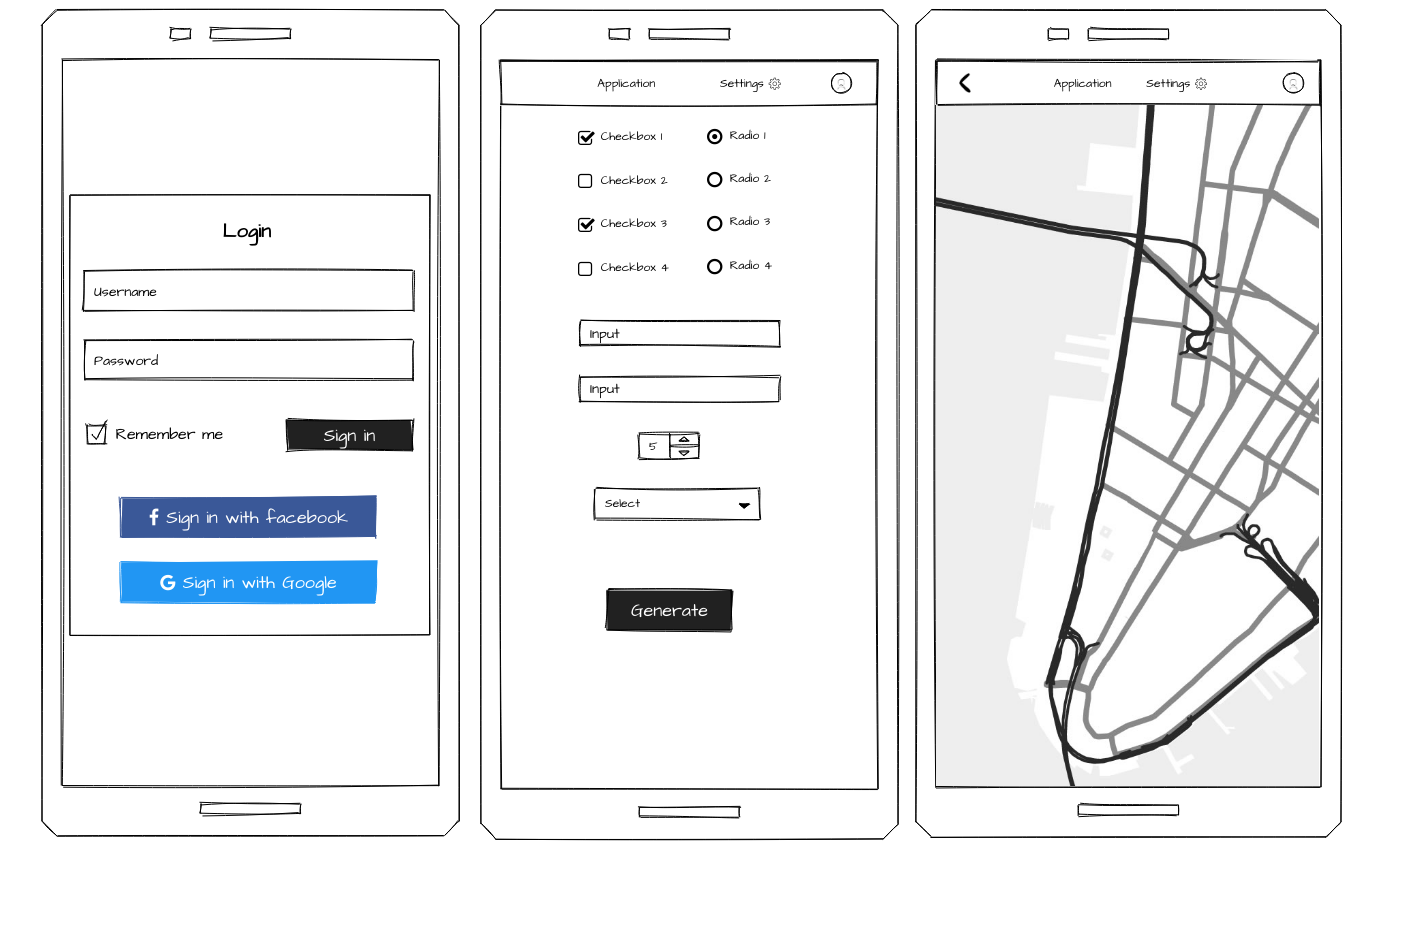
\includegraphics[width=\linewidth]{./graphics/wireframes.png}
    \caption{Wireframes.}
    \label{fig:wireframes}
\end{figure}

Figuur \ref{fig:wireframes} toont hoe de applicatie eruit zou kunnen zien. 
Dit is echter een eerste versie,
die nog verder uitgewerkt zal worden met behulp van de nodige analyse van huidige route-apps.
Het is de bedoeling dat een gebruiker/loopfanaat gemakkelijk een route kan genereren op basis van verschillende parameters. Deze route bevat dan ook een weersverwachting. 

%%---------- Andere bijlagen --------------------------------------------------
% TODO: Voeg hier eventuele andere bijlagen toe. Bv. als je deze BP voor de
% tweede keer indient, een overzicht van de verbeteringen t.o.v. het origineel.
%\input{...}

%%---------- Backmatter, referentielijst ---------------------------------------

\backmatter{}

\setlength\bibitemsep{2pt} %% Add Some space between the bibliograpy entries
\printbibliography[heading=bibintoc]

\end{document}
